% !TEX root = ../thesis-index.tex

\chapter{Fixed-points and global convergence of deep representations}
\label{ch:isometry_activation}

The study of neural networks has increasingly focused on understanding the internal mechanisms that govern their learning and generalization capabilities. A central aspect of this inquiry is how neural networks transform and preserve input data structure as it passes through multiple layers. One powerful approach to studying these transformations is through the lens of kernel methods, which have long been used in machine learning to understand the relationships between data points in high-dimensional spaces~\cite{scholkopf2002learning,smola2004tutorial}.

Studying neural networks from the perspective of kernels has been the subject of many theoretical studies. This perspective has led to significant advancements, such as the development of Neural Tangent Kernels (NTKs)~\cite{jacot2018neural} and Convolutional Kernel Networks~\cite{mairal2014convolutional}, or in the notion of dual kernel~\cite{daniely2016toward}. The idea that neural networks, especially in the infinite-width limit, can be understood through kernels has been explored in various recent works~\cite{lee2019wide, arora2019exact, yang2019scaling}. Moreover, the use of kernel methods to measure the similarity between inputs as the network processes them provides a powerful means of understanding the inductive biases and representative capacity of neural networks, particularly in the context of deep learning~\cite{zhang2017understanding,zhang2021understanding,cho2009kernel}.

However, the question of how the inner product between hidden layer representations evolves across layers and whether it converges globally to a fixed point remains an important but underexplored area of study~\cite{saxe2013exact, schoenholz2016deep, pennington2018emergence}. While previous research has provided insights into local behaviors~\cite{yang2018a}, a global analysis of fixed points and convergence properties of kernel sequences, particularly in the presence of nonlinear activations, still needs to be improved.

This chapter addresses this gap by introducing and analyzing the evolution of the kernel through layers. The kernel sequence tracks the similarity between two inputs. More concretely, we consider the kernel sequence $k(h^\ell(x), h^\ell(y)),$ where $k$ denotes some notion of similarity, such as inner product or cosine similarity, and $h^\ell(x)$ and $h^\ell(y)$ denote layer $\ell$ representation for respective inputs $x$ and $y$. Understanding whether and how this sequence converges to a fixed point as the network depth increases is crucial for uncovering the inherent implicit biases of deep networks.

Our analysis builds upon foundational work in understanding the role of activation functions in neural networks, such as the use of ReLU and its variants~\cite{glorot2011deep, nair2010rectified} and the exploration of nonlinear activations in large-scale models~\cite{ramachandran2017searching, clevert2015fast}. Additionally, the interplay between activation functions and normalization techniques, such as layer normalization~\cite{ba2016layer}, plays a critical role in shaping the convergence behavior of kernel sequences~\cite{klambauer2017self, hayou2019impact}. Moreover, the study of neural networks through the lens of kernel methods is deeply connected to earlier work on Gaussian processes~\cite{williams2006gaussian} and the dynamics of signal propagation in deep networks~\cite{poole2016exponential, raghu2017expressive}. By analyzing how these kernels evolve across layers, particularly in terms of activation functions, we contribute to a deeper understanding of the dynamics within deep neural networks.

Throughout this chapter, we assume that the network operates under the mean field regime, which simplifies the analysis by tending width to infinity and making stochastic sequences deterministic. 

\section{Preliminaries}
In this section, we introduce the fundamental concepts, notations, and definitions used throughout this chapter. 

We consider a feed-forward neural network with $L$ layers, each with width $d$. The network takes an input vector $x \in \mathbb{R}^d$ and maps it to an output vector $h^L(x) \in \mathbb{R}^d$ through a series of transformations. The hidden representations at each layer $\ell$ are denoted by $h^\ell(x)$. The transformation at each layer is composed of a linear transformation followed by a nonlinear activation function $\phi$. Mathematically, the hidden representation at layer $\ell$ is given by:
\begin{align}
& h^\ell(x) = \phi(W^\ell h^{\ell-1}(x)), && W^\ell \in \mathbb{R}^{d \times d},
\end{align}
where $h^0(x):=x$ is set to input, and elements of $W^\ell$ are drawn i.i.d. from $N(0,1/d)$. The activation function $\phi: \mathbb{R} \to \mathbb{R}$ denotes the activation applied element-wise. 
In some variations of the MLP, we will use normalization layers to adjust the activations at each layer, namely Layer Normalization (LN) or Root Mean Squared (RMS) normalization. Finally, the neural kernel between two inputs $x$ and $y$ at layer $\ell$ is defined as:
\begin{align}
    \rho_\ell = \frac{\langle h^\ell(x), h^\ell(y) \rangle}{\|h^\ell(x)\| \|h^\ell(y)\|},
\end{align}
where $\langle \cdot, \cdot \rangle$ denotes the inner product, and $\rho_0$ corresponds to similiarty between input samples $x$ and $y$.

The main goal of this chapter is to analyze sequence $\{\rho_\ell\},$ at initialization, when the weights are still random. The motivation for this analysis is to understand if various architectural choices, namely activation or number of layers, lead to specific biases of the kernel towards a certain fixed point. Namely, if there is a bias towards zero, it would imply that at initialization, the representations become more orthogonal. In contrast, a positive fixed point would mean the representations become more similar.

In the current setup, the sequence $\{\rho_\ell\}$ is a stochastic sequence or a Markov chain due to the random weights at each layer. 
However, we will show that under the mean field regime, the sequence $\{\rho_\ell\}$ converges to a deterministic sequence, and we will analyze the properties of this deterministic sequence.


\section{Mean field regime}

In this section, we conduct a mean field analysis of multilayer perceptrons (MLPs) to explore the neural kernel's fixed-point behavior as the network depth increases. This approach allows us to gain insight into the global dynamics of neural networks, mainly how the similarity between two input samples evolves as they pass through successive network layers.
Now, we can state the mean field regime for the kernel sequence, stating that in this regime, the sequence becomes deterministic.

\begin{proposition}
\label{iso:prop:mean_field_kernel}
Under the mean field regime, i.e., $d \to \infty$, the kernel sequence $\rho_\ell$ of an MLP with activation $\phi$ that obeys $\E_{X\sim N(0,1)} \phi(X)^2=1.$ Then the sequence evolves deterministically as follows:
\begin{align*}
&\rho_{\ell} = \mathbb{E}_{X,Y}[\phi(X)\phi(Y)], && 
\text{where } X, Y\sim N(0,1),\; \E XY = \rho_{\ell-1}.
\end{align*}
where the initial value $\rho_0$ corresponds to the input. 

\end{proposition}

Historically, conditions similar to $\E \phi(X)^2=1$ have been used to prevent the forward pass from vanishing or exploding. For example, applying ReLU will zero out half of the activations, which will lead to a vanishing norm of forward representations, and Kaiming He's initialization~\citet{he2016deep} addresses that by scaling weights to maintain consistent forward pass norms across layers. This principle is further refined in a self-normalizing activation~\citet{klambauer2017self}, ensuring consistent mean and variances between pre- and post-activations. 


\begin{proof}
 The proof is a straightforward application of the law of large numbers, as the mean field regime implies that the sample means converge to the population means. Let us inductively assume that at layer $\ell$ the it holds that $\frac1d\|h^{\ell}(x)\|^2 = 1$ and $\frac1d\|h^{\ell}(y)\|^2=1,$ and $\frac1d\langle h^{\ell}(x),h^{\ell}(y)\rangle = \rho_{\ell}$. Thus, if $X$ and $Y$ denote the pre-activations for a given unit for the two inputs at layer $\ell$, they follow standard Gaussian distribution and have covariance $\rho_{\ell}.$ By construction we have $\E \phi(X)^2 = \E \phi(Y)^2 = 1$, and $\E \phi(X)\phi(Y) = \rho_{\ell+1}.$ Finally, since each hidden unit is independent of others, based on the law of large numbers, we can conclude the samples means will converge to their expectation $\frac1d \|h^{\ell+1}(x)\|^2 = 1, $ $\frac1d \|h^{\ell+1}(y)\|^2 = 1,$ and $\frac1d \langle h^{\ell+1}(x),h^{\ell+1}(y)\rangle = \rho_{\ell+1}. $ This concludes the proof. 
\end{proof}

As you can see, this proposition shows that the kernel sequence $\rho_\ell$ converges to a deterministic sequence. We can relax the conditions on the weights to allow any distribution with zero mean and variance $1/d,$ such as uniform distribution. 

\begin{proposition}
\label{iso:prop:mean_field_kernel_general}
Under the mean field regime, i.e., $d \to \infty$, the kernel sequence $\rho_\ell$ of an MLP with activation $\phi$ that obeys $\E \phi(X)^2=1.$ If each element of the weights is drawn i.i.d. from a distribution with zero mean and $1/d$ variance, then the sequence evolves deterministically as given by Proposition~\ref{iso:prop:mean_field_kernel}.
\end{proposition}

\begin{proof}
 The key observation is that the pre-activations to each unit can be written as the sum of i.i.d. elements; by Central Limit Theorem, we can conclude that as $d\to\infty,$ their distribution converges to a normal distribution, which allows us to apply Proposition~\ref{iso:prop:mean_field_kernel}.
\end{proof}




Propositions \ref{iso:prop:mean_field_kernel} and \ref{iso:prop:mean_field_kernel_general} under the condition that under some normality conditions on activations,  showed the sequence evolution is entirely determined by a single parameter $\rho_{\ell-1}$, which evolves deterministically, 
Inspired by this property, we define it as the mapping between the covariance of pre-activations and the covariance of post-activations.

\begin{definition}
    \label{iso:def:kernel_map}
Given two random variables $X, Y$ with covariance $\rho,$ and activation $\phi,$ define the \emph{kernel map } $\kappa$ as the mapping between the covariance of pre-activations and the covariance of post-activations:
\begin{align}\label{iso:eq:kernel_map}
    \kappa(\rho):=\E_{X,Y}[ \phi(X)\phi(Y)], && \text{where } X, Y\sim N(0,1),\; \rho:=\E XY.
\end{align}
\end{definition}

With this definition, we can express the result of Propositions~\ref{iso:prop:mean_field_kernel} and~\ref{iso:prop:mean_field_kernel_general} in terms of the kernel map. Under the same setting as Proposition~\ref{iso:prop:mean_field_kernel_general}, the kernel sequence $\{\rho_\ell\}$ evolves deterministically according to the kernel map $\kappa$:
\begin{align}
    \rho_{\ell} = \kappa(\rho_{\ell-1}),
\end{align}
where $\kappa$ is defined in Definition~\ref{iso:def:kernel_map}.  Thus, in order to understand the convergence of sequence $\{\rho_\ell\},$ we can study the fixed-points of the kernel map $\kappa,$
which are the values of $\rho^*$ that satisfy $\kappa(\rho^*) = \rho^*.$ With the assumptoin that $\E \phi(X)^2=1,$ the kernel map $\kappa$ is a mapping between $[-1,-1]$ to itself. Thus, Brower's fixed-point theorem implies that the kernel map $\kappa$ has at least one fixed point $\rho^*.$ But as we will show, there is potentially more than one fixed point, and it will be interesting to understand which ones are locally or globally attractive. 


\section{Hermite expansion of activation functions}
Hermite polynomials possess completeness and orthogonality under the Gaussian weight kernel. This means that any function in the space of square-integrable functions with respect to the Gaussian kernel can be expressed as a linear combination of Hermite polynomials. The square integrability of an activation function ensures that it does not lead to exploding activations, as non-square integrable functions suggest heavy-tailed post-activations that lack second moments, and it holds for all activations that are used in practice. We use the \emph{normalized} Hermite polynomials and their coefficients. 

\begin{definition}
Define normalized Hermite polynomials $\he_k(x)$ as a scaled version of the probabilist's Hermite polynomials $\He_k(x)$, as follows
\begin{align*}
&\He_k(x) :=(-1)^k e^{x^2/2} \frac{d^k}{dx^k} e^{-x^2/2}, && \he_k(x):=\frac{1}{\sqrt{k!}} \he_k(x).
\end{align*}
\end{definition}

Here is a list of the first few normalized Hermite polynomials:

\begin{table}[ht]
    \centering
    \caption{Hermite polynomials and their normalized versions}
    \begin{tabular}{|c|c|c|c|c|c|}
    \hline
 Order & $k=0$ & $k=1$ & $k=2$ & $k=3$ & $k=4$ \\
 \hline
 $\He_k(x)$ & $1$ & $x$ & $ (x^2 - 1)$ & $(x^3 - 3x)$ & $(x^4 - 6x^2 + 3)$ \\    
 \hline
 $\he_k(x)$ & $1$ & $x$ & $\frac{1}{\sqrt{2}} (x^2 - 1)$ & $\frac{1}{\sqrt{6}} (x^3 - 3x)$ & $\frac{1}{\sqrt{24}} (x^4 - 6x^2 + 3)$ \\
    \hline
    \end{tabular}
\end{table}

Most importantly, Hermite polynomials satisfy the orthogonality property:
\begin{align}\label{iso:eq:hermite_orthogonality}
    &\E_{x\sim N(0,1)} \left[\He_k(x)\He_l(x)\right] = k! \delta_{kl}, &&\E_{x\sim N(0,1)} \left[\he_k(x)\he_l(x)\right] = \delta_{kl},
\end{align}
where $\delta_{kl}$ is the Dirac delta. Here we can see the motivation behind our normalization, as it cancels out with the factorial term in the orthogonality property. 

Based on this property, we can express any function $\phi$ as a linear combination of Hermite polynomials:

\begin{definition}\label{iso:def:hermite_expansion}
Given an activation function $\phi$ that is square-integrable with respect to the Gaussian kernel $\int_{-\infty}^\infty \phi(x)^2 e^{-x^2/2}dx < \infty$, the Hermite expansion of $\phi$ is defined as:
\begin{align*}
\phi(x) = \sum_{k=0}^\infty c_k \he_k(x),&&c_k = \E_{X\sim N(0,1)} \left[\phi(X) \he_k(X)\right],
\end{align*}
where $\he_k(x)$ are the normalized Hermite polynomials and $c_k$ are the Hermite coefficients. 
\end{definition}

% Based on the orthogonality of Hermite polynomials, we can make a few observations about some of the Hermite coefficients.  

Besides orthogonality, Hermite polynomials have another magical property that is crucial for our later analysis. 

\begin{lemma}[Consequence of Mehler's kernel]\label{iso:lem:mehler_kernel}
If $X,Y \sim N(0,1)$ with covariance $\E XY = \rho$ we have 
$$\E_{X,Y} \he_n(X)\he_k(Y) = \rho^n \delta_{nk}$$
where $\delta_{nk}$ is the Dirac delta.  
\end{lemma}

This lemma states that given two Gaussian random variables $X, Y$ with covariance $\rho,$, the expectation of the product of Hermite polynomials is zero unless the indices are equal. 

\begin{proof}[Proof of Lemma~\ref{iso:lem:mehler_kernel}]
The property can be deduced from Mehler's formula~\cite{mehler1866ueber}. The formula states that 
\begin{align*}
&\frac{1}{\sqrt{1-\rho^2}}\exp\left(-\frac{\rho^2(x^2+y^2)-2xy\rho}{2(1-\rho^2)}\right) \\
&= \sum_{m=0}^\infty \he_m(x)\he_m(y),
\end{align*}
where the $m!$ factor difference is due to the definition of Hermite polynomials with an additional $1/\sqrt{m!}$ compared to the one used in Mehler's kernel. 
Observe that the left-hand side is equal to $p(x,y)/p(x)p(y)$, where $p(x,y)$ is the joint PDF of $(X, Y)$, and $p(x),p(y)$ are PDF of $X$ and $Y$ respectively. Therefore, we can take the expectation using the expansion 
\begin{align*}
\E_{X,Y}\left[ \he_n(X) \he_k(Y)\right] &= \int \he_n(x)\he_k(y)p(x,y)dx dy \\
&=  \sum_{m=0}^\infty \rho^m\int \he_n(x)\he_k(y) \he_m(x)\he_m(y) dp(x)dp(y)\\
&= \sum_{m=0}^\infty \rho^m\E_{X\sim N(0,1)} \left[\he_n(X)\he_m(X)\right]\E_{Y\sim N(0,1)} \left[\he_k(Y)\he_m(Y)\right] \\
&= \rho^n \delta_{nk} 
\end{align*}
where in the last line we used the orthogonality property $\E_{X\sim N(0,1)} H_k(x) H_n(X)=\delta_{nk}$. 
\end{proof}

Lemma~\ref{iso:lem:mehler_kernel} is crucial for our theory. Based on this lemma, we can express the kernel map in terms of the Hermite coefficients, showing a particular structure of the kernel map.

\begin{corollary}
    \label{iso:cor:hermite_covariance}
    \label{iso:cor:kernel_map}
Given $X,Y \sim N(0,1)$ with covariance $\E X Y = \rho,$ and $\phi(X) = \sum_{k=0}^\infty c_k \he_k(X),$ we have
\begin{align*}
\kappa(\rho) = \E_{X\sim N(0,1)} \left[\phi(X)\phi(X)\right] = \sum_{k=0}^\infty c_k^2 \rho^k.
\end{align*}
\end{corollary}

\begin{proof}[Proof of Corollary~\ref{iso:cor:hermite_covariance}]
Using Lemma~\ref{iso:lem:mehler_kernel} we have
\begin{align*}
\E_{X\sim N(0,1)} \left[\phi(X)\phi(X)\right] = \E_{X\sim N(0,1)} \left[\sum_{k=0}^\infty c_k \he_k(X)\sum_{l=0}^\infty c_l \he_l(X)\right] = \sum_{k=0}^\infty c_k^2 \rho^k.
\end{align*}
\end{proof}

These algebraic properteis of kernel map will be crucial in our analysis of the convergence of the kernel sequence to a fixed point. Before we turn our attention to convergence, let us draw some links between the properties of activation functions, its kernel map, and its Hermite coefficients.

\begin{table}[ht]
    \centering
    \caption{Properties of activations in terms of Hermite coefficients and kernel map}
    \begin{tabular}{|c|c|c|c|}
    \hline
 Property & Activation $\phi$ & Hermite coefficients $\{c_k\}_{k\ge 0}$ & Kernel map $\kappa$ \\
    \hline
 Centered & $\E \phi(X)=0$ & $c_0 = 0$ & $\kappa(0) = 0$ \\
    \hline
 Stable & $\E \phi(X)^2 = 1$ & $\sum_{k=0}^\infty c_k^2 = 1$ & $\kappa(1) = 1$ \\
    \hline
 Non-linear & $\phi(x)$ is non-linear & $\sum_{k=2}^\infty c_k^2 > 0$ & $\kappa(\rho)$ is non-linear \\
    \hline
    \end{tabular}
\end{table}


\section{Globally contracting kernel to zero}

Recall that for activations that obey $\E \phi(X)^2 = 1,$, the kernel map  $\kappa$ is a power series with non-negative coefficients $\sum_k c_k \rho^k$ that maps $[-1,1]$ to itself, and obeys $\kappa(1)=1.$ This immediately reveals that $\rho=1$ is a fixed point of the kernel map. This is unsurprising, as it reaffirms the fact that if two inputs are identical with unit variance, the post-activations will also be identical. However, it is far more interesting whether this fixed point is globally attractive and how the kernel map influences the convergence rate to this fixed point. In a similar vein, we can ask if there are other fixed points and how the kernel map influences the convergence rate to these fixed points.

In the same vein as previous chapters, we are primarily interested in seeing which properties in the kernel maps lead to convergence towards orthogonality. In other words, we are primarily interested in conditions that lead to $\rho^*=0$ being a fixed point and under which conditions this fixed point is globally attractive. 



% A quantity that will be crucial for our analysis is the contraction rate of the kernel map, which is defined based on the Hermite coefficients of the activation function.

% \begin{definition}
%     \label{iso:def:contraction_rate}
%  Given activation $\phi$ that with Hermite coefficients $\{c_k\}_{k\ge 0},$ it contraction rate $\alpha$ is defined as:
%     \begin{align}\label{iso:eq:contraction_rate}
%         \alpha = \frac{\sum_{k=1}^\infty c_k^2}{\sum_{k=1}^\infty  k c_k^2 } = \frac{\kappa(1)-\kappa(0)}{\kappa'(1)}.
%     \end{align}
% \end{definition}

% We can make the following important observation about the range and extreme values of the contraction rate $\alpha.$

% \begin{remark}
%     \label{iso:rem:contraction_rate}
%  Note that the term 
%     $(\sum_{k=1}^\infty c_k^2)/(\sum_{k=1}^\infty k c_k^2)$
%  is always in the range $[0,1].$ Furthermore, $\alpha < 1$ if and only if the activation is non-linear, i.e., $c_k \neq 0$ for some $k\ge 2.$ We can also observe this from the second formulation: the numerator $(\kappa(1)-\kappa(0))/(1-0)$ encodes the slope of the line connecting $(0,\kappa(0))$ and $(1,\kappa(1)),$ and the denominator $\kappa'(1)$ is the slope of the tangent line at $\rho=1.$ Because $\kappa$ is convex in $[0,1]$ the tangent slope is higher than the line slope, which implies $\alpha\le 1,$ and it becomes strict if and only if the convexity is strict, i.e., the activation is non-linear. 
% \end{remark}


Finally, we can state one of the central results of this chapter, which characterizes the global convergence of the kernel map towards the fixed point $\rho^*=0.$

\begin{theorem}\label{iso:thm:global_attract}
Let $\phi$ be an activaiton with kernel map $\kappa$ that is centered $\kappa(0)=0,$ and $\kappa(1)=1.$ Let $\rho_\ell$ be the kernel sequence $\rho_{\ell+1}=\kappa(\rho_\ell),$ given initial value $\rho_0.$ Then, the sequence contracts towards fixed-point zero $\rho^*=0$ with rate $\alpha$:
    \begin{align}
        &\frac{|\rho_\ell|}{1-|\rho_\ell|} \le \frac{|\rho_0|}{1-|\rho_0|}\alpha^{\ell}, && \alpha := \frac{1}{2-\kappa'(0)},
    \end{align}
 where $\alpha$ is strictly less than one if the activation is non-linear. The only other fixed points can be $\rho^*=1$ or $\rho^*=-1,$, and none of them is locally or globally attractive.
\end{theorem}

Note that the statement becomes vacuous if the initial covariance is $\rho_0 = 1$ or $\rho_0 = -1$, as in these cases, the right-hand side goes to infinity, but the theorem is non-vacuous for all $\rho_0\in(-1,1).$ This is unsurprising, as the kernel map cannot separate the two inputs if they are identical or anti-identical. In plain words, this states that if the two samples are not identical, by iteratively passing them through a nonlinear activation, the covariance between them will contract with rate $\alpha$ in expectation.  While it may not seem immediately obvious why $\alpha < 1$ for non-linear activations, the following remark makes the connection between the two.

\begin{remark}
    \label{iso:rem:contraction_rate}
    Let us assume $\kappa(\rho)=\sum_{k=0}^\infty c_k^2\rho^k,$ where $c_k$ denote Hermite coefficients. Note that $\kappa'(0) = c_1^2 \le \sum_{k=0}^\infty c_k^2 = \kappa(1)=1$. Now, if we have $\kappa'(1)=1,$ it implies that $c_k=0$ for all $k\ge 2.$ This is a contradiction with the assumption that the activation is non-linear.  
\end{remark}


Another observation is that rather than proving convergence directly, we showed contraction under the potential $|\rho|/(1-|\rho|).$ Because $|\rho|/(1-|\rho|)$ is a monotonically increasing with $|\rho|$, the contraction of $|\rho_\ell|/(1-|\rho_\ell|)$ implies contraction of $|\rho_\ell|$ towards zero. We can state the contraction directly in terms of the sequence $\rho_\ell $.

\begin{corollary}
Under the same setting as in Theorem~\ref{iso:thm:global_attract}, the sequence $\rho_\ell = \kappa(\rho_{\ell-1})$ converges to zero with rate $|\rho_\ell| \le \rho_0/(1-|\rho_0|) \alpha^{\ell}$.
\end{corollary}

The proof follows directly from Theorem~\ref{iso:thm:global_attract} and the inequality $|\rho_\ell| \le |\rho_\ell|\le (1-|\rho_\ell|).$ 


% We can now state and prove the main theorem of this section, which characterizes the global convergence of the kernel map towards the fixed point $\rho^*=0.$

% \begin{theorem}\label{iso:thm:global_attract}
%  Consider activation $\phi,$ that with Gaussian pre-activations, has zero mean $\E_{X}\phi(X)=0$ and unit variance $\E_{X}\phi(X)^2 = 1,$ the sequence $\rho_\ell = \kappa(\rho_{\ell-1})$ contracts towards zero with rate $\alpha$:
%     \begin{align}
%         \Psi(\rho_\ell)\le \Psi(\rho_0) \alpha^{\ell}, 
%     \end{align}
%  where $\alpha$ is defined in \eqref{iso:eq:contraction_rate}, which becomes strictly less than one if the activation is non-linear. 
% \end{theorem}

\textit{Proof idea:} The main proof idea of this theorem is to show that upon applying the kernel map $\kappa$ to the covariance of pre-activations, the potential function $|\rho|/(1-|\rho|)$ decreases with rate $\alpha,$ and applying an induction over $\ell.$ Condition $\kappa(1)=\E \phi(X)^2 = 1$ ensures that activations are stable and do not explode or vanish, allowing us to apply the single step contraction inductively. The proof of the single step follows from the properties of Hermite polynomials and the orthogonality of the kernel map. The non-linearity condition is essential to have $\alpha<1,$ which rules out identity-like activations that do not change the value. The centered condition $\kappa(0)=\E \phi(X) = 0$ ensures that $\rho^*$ is a fixed point.

Some activations, such as SeLU~\citet{klambauer2017self}, which is a self-normalizing activation function that has $\E \phi(X)^1 = 0.$ 

% \begin{proof}
% The proof follows directly from Proposition~\ref{iso:prop:isometry_bias}, by applying induction over $\ell.$
% \end{proof}


\begin{proof}[Proof of Theorem~\ref{iso:thm:global_attract}]
 The main technical part of the proof is to prove that:
    \begin{align*}
        \Psi(\kappa(\rho)) \le \alpha \Psi(\rho), && \Psi(\rho) = \frac{|\rho|}{1-|\rho|}.
    \end{align*}
Base don the given assumptions we have $c_0^2 = \kappa(0) = 0$ and based on the assumption $\E \phi^2(X)=1$ and properties of Hermite polynomials we have $\kappa(1)=\sum_{k=1}^\infty c_k^2 = 1.$ 
    
 First, we will consider positive $\rho\in[0,1),$ for which we have
    \begin{align*}
 \frac{\Psi(\kappa(\rho))}{\Psi(\rho)}&=\left(\frac{\kappa(\rho)}{1-\kappa(\rho)}\right)  \left(\frac{\rho}{1-\rho}\right)^{-1}\\  
        &= \frac{\rho^{-1}\sum_{k=1}^\infty c_k^2 \rho^{k} }{(1-\rho)^{-1}\sum_{k=1}^\infty c_k^2 (1-\rho^{k})} \\
        &= \frac{\sum_{k=1}^\infty c_k^2 \rho^{k-1}}{\sum_{k=1}^\infty c_k^2 \left(\frac{1-\rho^{k}}{1-\rho}\right)}\\
        &= \frac{\sum_{k=1}^\infty c_k^2 \rho^{k-1}}{\sum_{k=1}^\infty c_k^2 \left(\sum_{i=0}^{k-1}\rho^{i}\right)}\\
        &\le \frac{\sum_{k=1}^\infty c_k^2\rho^{k-1} }{\sum_{k=1}^\infty c_k^2 \rho^{k-1} + \sum_{k=2}^\infty c_k^2}\\
        &\le \max_{\rho\in[0,1]} \frac{\sum_{k=1}^\infty c_k^2\rho^{k-1} }{\sum_{k=1}^\infty c_k^2 \rho^{k-1} + \sum_{k=2}^\infty c_k^2}\\
        &= \frac{\sum_{k=1}^\infty c_k^2}{2\sum_{k=1}^\infty c_k^2 -c_1^2 } \\
        &=\frac{1}{2-\kappa'(0)} =: \alpha.
    \end{align*}
 Now, we can use the fact that the norm of the sum of values is bounded by the sum of their norms to argue that
    \begin{align*}
 |\kappa(\rho)|=|\sum_{k=1}^\infty c_k^2 \rho^k | &\le \sum_{k=1}^\infty c_k^2 |\rho|^k 
 = \kappa(|\rho|)
    \end{align*}
 Because $x\mapsto x/(1-x)$ is monotonically increasing for $x\in[0,1]$, for all $\rho\in[-1,1]$ we have 
    \begin{align*}
 \frac{|\kappa(\rho)|}{1-|\kappa(\rho)|}\le \frac{\kappa(|\rho|)}{1-\kappa(|\rho|)} \le \frac{|\rho|}{1-|\rho|}\alpha.
    \end{align*}
Where we invoked the inequality that was proven for $\rho\in[0,1], $ Plugging in the definition of $\Psi$ we have proven that for all $\rho$ we have
\begin{align*}
    \Psi(\kappa(\rho)) \le \alpha \Psi(\rho).
\end{align*}
We can conclude the proof by induction over $\ell.$

\textit{Other fixed-points:}
What remains to show is that the only possible fixed points are $\rho^*=0,1,-1,$, and only $1,-1$ are neither locally or globally attractive.  

First, by contraction result we have so far, for any $\rho \in (-1,1),\rho\neq 0,$ then $|\kappa(\rho)|$ will be strictly smaller than $|\rho|,$ which contradicts with it being a fixed point. That only leaves $\{-1,0,1\}$ as possible fixed points. Now, we will prove that $-1,1$ are not locally attractive fixed points. 

For $\rho^*=1$ to be locally attracting, we must have $|\kappa'(\rho^*)|<1,$ and by construction we have $\kappa'(0)<1,$ However, this implies in some small $\epsilon$ there is $\rho_0\in(0,\epsilon)$ and $\rho_1 \in (1-\epsilon,1),$ such that we have $\kappa(\rho_0) < \rho_0$ and $\kappa(\rho_1) > \rho_1.$ Now, by continuity of $\kappa(\rho)$ there must be a point $\rho_2\in (\rho_0,\rho_1)$ such that $\kappa(\rho_2) = \rho_2,$ which contradicts the assumption that $\rho^*=1$ is the only fixed point. The same argument can be made for $\rho^*=-1.$ 

Thus, we have shown that only $\{-1,0,1\}$ can be fixed-point, and only $\rho^*=0$ is globally attractive.
\end{proof}



\section{Convergence of the kernel with general activations}
So far, we only discussed the convergence of the kernel map for activations that are centered and the convergence of their kernel sequence towards zero. However, we can extend this analysis to general activations that are not centered. In this section, we will show that for any activation function that is non-linear, there is a unique fixed point $\rho^*$ that is globally attractive.


\begin{theorem}
Let $\kappa$ be the kernel map satisfying $\kappa(1)=1$. Define the kernel sequence $\rho_{\ell+1}=\kappa(\rho_\ell)$, with initial step $\rho_0 \in (-1,1)$. Assuming that the activation is non-linear, there is a unique $\rho^*$ that is globally contracting, which is necessarily non-negative $\rho^*\in[0,1].$ The only other fixed-points distinct from $\rho^*,$ could be $-1$ or $1,$ neither of which are locally or globally contracting. Furthermore, we have the following contraction rate towards $\rho^*$:
\begin{enumerate}
    \item If $\kappa(0)=0$, then $\rho^*=0$ is an attracting with rate 
    \begin{align}
    \frac{|\rho_\ell|}{1-|\rho_\ell|} \le \frac{|\rho_0|}{1-|\rho_0|} (1/\kappa'(1))^\ell
    \end{align}
    \item If $\kappa(0)>0$ and $\kappa'(1)<1$, then $\rho^*=1$ is an attracting, with rate 
    \begin{align}
    |\rho_\ell-1| \le |\rho_0-1| (\kappa'(1))^\ell
    \end{align}
    \item If $\kappa(0) > 0$, and $\kappa'(1)=1$ then  $\rho^*=1$ is attracting with rate 
    \begin{align}
    |\rho_\ell-1| \le \frac{|\rho_0-1|}{\ell\alpha|\rho_0-1|+1}, && \alpha = 1-\kappa(0)-\kappa'(0).
    \end{align}
    \item If $\kappa(0) > 0$, and $\kappa'(1)>1$ then the attracting fixed point is necessarily in the range $\rho^*\in(0,1)$, we have  
    \begin{align}
    &|\rho_\ell-\rho^*| \le \frac{|\rho_0-\rho^*|}{1-|\rho_0|}\alpha^\ell && \alpha = \max\left\{1-\kappa(0),\kappa'(\rho^*),\frac{1-\rho^*}{2-\kappa'(\rho^*)}\right\},
    \end{align}
    where $\alpha$ is strictly less than one if the activation is non-linear.
\end{enumerate}
\end{theorem}

\begin{remark}
One of the most striking results of this theorem is that for any non-linear activation, there is a unique fixed point $\rho^*$ that is locally or globally attractive. Furthermore, the fixed point is necessarily non-negative. This implies that for any MLP with non-linear activations, the covariance of pre-activations will converge towards a fixed point, which is always non-negative. 
\end{remark}

\begin{remark}
The assumptions laid out in the theorem are nearly tight. For example, the non-linearity assumption is necessary to rule out identity activation, where every point in $[-1,1]$ is a fixed point. Furthermore, considering odd activations such as $\phi(x) = x^3,$ and we can see that if $\rho_0\in\{-1,1\}$, the sequence will remain the same $\rho_\ell=\rho_0,$ and hence will not converge, which implies the condition that $\rho_0\in(-1,1)$ is necessary. 
\end{remark}

\begin{remark}
Note that all convergence rates are of exponential form $\|\rho_\ell-\rho^*\|= O(\alpha^\ell),$ where $\alpha<1$ if the activation is non-linear, with the exception of the case where $\kappa'(1)=1,$ where the rate is of the form $O(1/\ell).$ 
\end{remark}

\begin{proof}
We will cases individually, starting with the first case that falls direclty under a previous theorem. 

\subsection*{Case 1: $\kappa(0)=0$}
We can observe that the case where $\kappa(0)=0,$ falls directly under Theorem~\ref{iso:thm:global_attract}, and thus there is no need to prove it again.

\subsection*{Cases 2,3: $\kappa(0)>0$ and $\kappa'(1)\le 1$} In this part, we jointly consider two cases where $\kappa(0)>0$ and $\kappa'(1) < 1,$ and $\kappa'(1)=1.$ Let us consider the ratio between distances $|\rho_\ell-1|$:
\begin{align*}
    \frac{|\kappa(\rho)-1|}{|\rho-1|} &= \frac{1-\kappa(\rho)}{1-\rho} \\
    &=\frac{\kappa(1)-\kappa(\rho)}{1-\rho}\\
    &=\frac{\sum_{k=1}^\infty c_k^2 (1-\rho^k)}{1-\rho}\\
    &=\sum_{k=1}^\infty c_k^2 \sum_{i=0}^{k-1}\rho^i\\
\implies \frac{|\kappa(\rho)-1|}{|\rho-1|} &=\kappa'(1)-\kappa'(1)+\sum_{k=1}^\infty c_k^2 \sum_{i=k}^\infty \rho^i\\
&= \kappa'(1)-\sum_{k=1}^\infty c_k^2 \big(k-\sum_{i=k}^\infty \rho^i\big)\\
\end{align*}
Clearly, the term $k-\sum_{i=k}^\infty \rho^i$ is is always non-negative, implying that if $\kappa'(1)<1$ we have the contraction 
\begin{align*}
    \frac{|\kappa(\rho)-1|}{|\rho-1|} \le \kappa'(1) \implies |\rho_\ell-1| \le |\rho_0-1| \kappa'(1)^\ell.
\end{align*}
Otherwise, if $\kappa'(1)=1,$ we have 
\begin{align*}
    \frac{|\kappa(\rho)-1|}{|\rho-1|} = 1-\sum_{k=1}^\infty c_k^2 \big(k-\sum_{i=0}^{k-1} \rho^i\big).
\end{align*}
Now, observe that the first term for $k=1$ is zero. Furthermore, the sequence $k-\sum_{i=0}^{k-1}\rho^i$ is monotonically increasing in $k$. Thus, the smallest value the weighted sum can achieve is if all of the weights of terms above $k\ge 2$ are concentrated in $k=2,$ which leads to the contraction
\begin{align*}
    \frac{|\kappa(\rho)-1|}{|\rho-1|} \le 1-(1-c_0^2-c_1^2)(2-1-\rho) = 1- (1-c_0^2-c_1^2) (1-\rho).
\end{align*}
Now, define sequence $x_\ell:= 1-\rho_\ell,$ and observe that we have 
\begin{align*}
    x_{\ell+1} \le x_\ell (1-\alpha x_\ell), && \alpha = 1-c_0^2-c_1^2,
\end{align*}
where $\alpha > 0$ if the activation is non-linear. 
We can prove inductively that 
\begin{align*}
x_\ell\le \frac{x_0}{\ell\alpha x_0 + 1}.
\end{align*}
If we plug in the definition of $x_n$ we have proven
\begin{align*}
|\rho_\ell-1| \le \frac{|\rho_0-1|}{\ell \alpha |\rho_0-1| + 1}.
\end{align*}

\subsection*{Case 4: $\kappa(0)>0$ and $\kappa'(1)>1$}
The main strategy is to prove some contraction of $\kappa(\rho)$ towards $\rho^*$, under the kernel map $\kappa$. In other words, we need to show $|\kappa(\rho)-\rho^*|$ is smaller than $|\rho-\rho^*|$ under some potential. First, we assume there is a $\rho^*$ such that $\kappa'(\rho^*)<1,$ and show this contraction, and later prove its existence and uniqeness. 

To prove contraction towards $\rho^*$ when $\kappa'(\rho^*)<1$, we consider three cases: 1) If $\rho > \rho^*$, 2) If $\rho \in [0,\rho^*]$, and 3) If $\rho < 0$. However, the bounds will be of different potential forms and will have to be combined later.  Let $\kappa(\rho) = \sum_{k=0}^\infty c_k^2 \rho^k$ be the kernel map with $\kappa(1)= 1$ with fixed-point $\rho^*$ that satisfies $\kappa'(\rho^*)<1.$

\begin{itemize}
\item \textbf{$\rho\ge \rho^*$.} we will prove:
\begin{align*}
\frac{|\kappa(\rho)-\rho^*|}{1-\kappa(\rho)} \le \frac{|\rho-\rho^*|}{1-\rho} \kappa'(\rho^*)
\end{align*}

We have the series expansion around $\rho^*$: $\kappa(\rho) = \rho^* + \sum_{k=1}^\infty a_k (\rho-\rho^*)^k$. For points $\rho\ge \rho^*$, we will have $\kappa(\rho)\ge \rho^*$, thus we can write

\begin{align*}
\frac{\kappa(\rho)-\rho^*}{1-\kappa(\rho)} &= \frac{\sum_{k=1}^\infty a_k (\rho-\rho^*)^k}{\kappa(1)- \kappa(\rho^*)}\\
&= \frac{\sum_{k=1}^\infty a_k (\rho-\rho^*)^k}{\sum_{k=1}^\infty a_k (1-\rho^*)^k - \sum_{k=1}^\infty a_k (\rho-\rho^*)^k}  \\
&= \frac{(\rho-\rho^*)\sum_{k=1}^\infty a_k (\rho-\rho^*)^{k-1}}{(1-\rho)\sum_{k=1}^\infty a_k (\sum_{i=0}^{k-1}(1-\rho^*)^i(\rho-\rho^*)^{k-1-i})} \\
&= \frac{\rho-\rho^*}{1-\rho}\cdot\frac{\sum_{k=1}^\infty a_k (\rho-\rho^*)^{k-1}}{\sum_{k=1}^\infty a_k (\sum_{i=0}^{k-1}(1-\rho^*)^i(\rho-\rho^*)^{k-1-i})}\\
&\le \frac{\rho-\rho^*}{1-\rho}\frac{\sum_{k=1}^\infty a_k (\rho-\rho^*)^{k-1}}{\sum_{k=2}^\infty a_k (1-\rho^*)^{k-1} + \sum_{k=1}^\infty a_k (\rho-\rho^*)^{k-1}}\\
&\le \max_{\rho\in[\rho^*,1]}\frac{\rho-\rho^*}{1-\rho}\frac{\sum_{k=1}^\infty a_k (\rho-\rho^*)^{k-1}}{\sum_{k=2}^\infty a_k(1-\rho^*)^{k-1} + \sum_{k=1}^\infty a_k (\rho-\rho^*)^{k-1}}\\
&\le \frac{\rho-\rho^*}{1-\rho}\frac{\sum_{k=1}^\infty a_k (1-\rho^*)^{k-1}}{\sum_{k=2}^\infty a_k (1-\rho^*)^{k-1} + \sum_{k=1}^\infty a_k (1-\rho^*)^{k-1}}\\
&=\frac{\rho-\rho^*}{1-\rho}\frac{\kappa(1)-\rho^*}{2\kappa(1)-\kappa'(\rho^*)}\\
&=\frac{\rho-\rho^*}{1-\rho}\frac{1-\rho^*}{2-\kappa'(\rho^*)}
\end{align*}
Thus, we have proven that 
\begin{align*}
\rho \ge \rho^* \implies \frac{|\kappa(\rho)-\rho^*|}{1-\kappa(\rho)} \le \frac{|\rho-\rho^*|}{1-\rho} \frac{1-\rho^*}{2-\kappa'(\rho^*)}
\end{align*}

% Now, because we can view the numerator and denominator as weighted sums, with $a_k$ as weights, and considering that the ratio between $(\rho-\rho^*)^{k-1}$ and $\sum_{i=0}^{k-1}(1-\rho^*)^i(\rho-\rho^*)^{k-1-i}$ is monotonically increasing in $\rho$, we can conclude that the ratio is maximized at $\rho$ is maximum, i.e., $\rho=1$. Thus, we can write
% \begin{align*}
% \rho \ge \rho^* \implies \frac{|\kappa(\rho)-\rho^*|}{1-\kappa(\rho)} \le \frac{|\rho-\rho^*|}{1-\rho} \frac{\sum_{k=1}^\infty a_k (1-\rho^*)^{k-1}}{\sum_{k=1}^\infty k a_k (1-\rho^*)^{k-1}} = \frac{|\rho-\rho^*|}{1-\rho} \frac{1-\rho^*}{\kappa'(1)}
% \end{align*}
% For the last step, we can recognize the quantities numerator quantity as $\kappa(1)-\rho^* = 1-\rho^*,$ while the denominator is $\kappa'(1)$. Thus, we have proven 
% \begin{align*}
% \rho \ge \rho^* \implies \frac{|\kappa(\rho)-\rho^*|}{1-\kappa(\rho)} \le \frac{|\rho-\rho^*|}{1-\rho} \frac{1-\rho^*}{\kappa'(1)}
% \end{align*}

\item \textbf{$0\le \rho \le \rho^*$.}
Consider $\rho \in [0,\rho^*]$. For these $\kappa'(\rho)$ is always monotonically increasing, implying that $\kappa'(\rho)\le \kappa'(\rho^*) < 1$. Thus, $|\kappa(\rho)-\rho^*| \le \kappa'(\rho^*) |\rho - \rho^*|$. This implies that in this range $|\kappa(\rho)-\rho^*|$ will contract with a rate $\kappa'(\rho^*)$:
\begin{align*}
0\le \rho \le \rho^* \implies |\kappa(\rho) - \rho^*| \le \kappa'(\rho^*) |\rho-\rho^*|
\end{align*}

\item \textbf{$-1 \le \rho \le 0$.}
Finally, let us consider $\rho \le 0$. Recall that we have $\kappa(1) = 1$. Thus, we can express $\kappa(\rho)-1$ as product of $(\rho-1)$ with some power series $q(\rho)$:
\begin{align*}
\kappa(\rho) - 1 = (\rho-1)q(\rho), \quad q(\rho) = \sum_{k=0}^\infty b_k \rho^k.
\end{align*}
In fact, we can expand $\kappa(\rho)$ in terms of these new coefficients
\begin{align*}
\kappa(\rho) = 1-b_0 + \sum_{k=0}^\infty (b_k - b_{k+1}) \rho^k
\end{align*}
Due to the non-negativity of coefficients of $\kappa$, we can conclude $1\ge b_0 \ge b_1 \ge ...$. Based on this observation, for $0 < \rho < 1$, we can conclude
$q(-\rho) = b_0 - b_1 \rho + b_2 \rho^2 - ... \le b_0$. Because we can pair each odd and even term $-b_{k}\rho^k + b_{k+1} \rho^{k+1}$ for all odd $k$, and because coefficients $b_k \ge b_{k+1}$ and $\rho^{k} \ge \rho^{k+1}$ for $\rho \in [0,1]$, we can argue $q(-\rho) \le b_0 = 1 - c_0^2$. Now, plugging this value into the kernel map for $0 < \rho < 1$, we have:
\begin{align*}
\kappa(-\rho) &= 1 - (1+\rho)q(-\rho) \\
&\ge 1-(1+\rho)(1-c_0^2)\\
&= 1 - 1 - \rho - c_0^2 (1+\rho)\\
&\implies \kappa(-\rho) + \rho \ge c_0^2 (1+\rho)\\
&\implies -\rho + c_0^2(1+\rho) \le \kappa(-\rho) \le \kappa(\rho)
\end{align*}
Now, if we assume $\kappa(-\rho) \le \rho^*$ then
\begin{align*}
\frac{|\kappa(\rho)-\rho^*|}{|-\rho-\rho^*|}=\frac{\rho^* - \kappa(-\rho)}{\rho^* + \rho} \le \frac{\rho^* + \rho - c_0^2 (1+\rho)}{\rho+\rho^*} = 1- \frac{c_0^2(1+\rho)}{\rho+\rho^*} \le 1-c_0^2
\end{align*}
Now, if we assume $\kappa(-\rho) \ge \rho^*$, knowing that $\kappa(-\rho)\le \kappa(\rho)$, which necessitates $\rho\ge \rho^*$, which implies $\kappa(\rho)\le \rho$. Thus, we have
\begin{align*}
\frac{|\kappa(-\rho)-\rho^*|}{|-\rho-\rho^*|} = \frac{\kappa(-\rho)-\rho^*}{\rho+\rho^*}\le \frac{\kappa(\rho)-\rho^*}{\rho+\rho^*} \le \frac{\rho-\rho^*}{\rho+\rho^*} \le \frac{1-\rho^*}{1+\rho^*} \le 1-\rho^*
\end{align*} 
Combining both cases we have 
\begin{align*}
\rho \le 0 \implies \frac{|\kappa(\rho)-\rho^*|}{|\rho-\rho^*|} \le 1 - \min(c_0^2 , \rho^*) = 1-\min(\kappa(0),\rho^*).
\end{align*}
We can further prove that $\rho^* = \kappa(\rho^*) = k(0) + \text{non-negative terms}$, which implies that $\rho^* \ge k(0)$. Thus, we can conclude that 
\begin{align*}
\rho \le 0 \implies |\kappa(\rho)-\rho^*| \le (1 - k(0))|\rho-\rho^*|
\end{align*}
\end{itemize}

\textbf{Positivity, uniqueness, and existence of a globally attractive fixed-point}
Here, the goal is to prove there is exactly one point $\rho^*\in[0,1]$ such that $\kappa(\rho^*) = \rho^*$ and $\kappa'(\rho^*) < 1.$ We will prove the properties of positivity, uniqueness, and existence separately.

\textit{Positivity:} Let us assume that $\rho^* \le 0.$ is a fixed-point. Then, we can apply the contraction rate proven for Case 3, which shows that $\kappa(\rho^*)\ge \rho^* + k(0) > \rho^*,$ which is a contradiction.


\textit{Uniqueness:} Assume that there are two fixed points $\rho_1$ and $\rho_2$ that satisfy $\kappa'(\rho_1),\kappa'(\rho_2)<1.$ Let us assume wlog that $\rho_1 < \rho_2.$ Then we can invoke the contraction rate proven so far to argue that all points in $(-1,1),$ including  $\rho\in (\rho_1,\rho_2)$ are attracted towards both $\rho_1$ and $\rho_2,$ which is a contradiction. Thus, there can be at most one fixed point.

\textit{Existence of $\rho^*$:} Because $\kappa(1)=1$ the set of all fixed-points is non-empty. Let us assume that $\rho^*$ is the first (smallest) fixed point of $\kappa(\rho^*) = \rho^*,$ which because of the positivity result is necessarily $\rho^*>0.$ If we assume that $\kappa'(\rho^*) > 1,$ then in the small $\epsilon$-neighborhood of it $\rho_1 \in(\rho^*-\epsilon,\rho^*)$ we have $\kappa(\rho_1) < \rho_1.$ Because $\kappa(\rho)$ is continuous, and is above identity line at $\rho=0$ and under identity line $\rho=\rho_1,$ there must be a point $0 < \rho_2 < \rho_1$ where it is at identity $\kappa(\rho_2) = \rho_2,$ which is a contradiction with assumption that $\rho^*$ is the smallest fixed point. Thus, we must have $\kappa'(\rho^*) \le 1.$ If we assume that $\kappa'(\rho^*) = 1,$ then the $\kappa$ must align with the identity line from $\rho^*$ to $1,$ which implies that all higher order terms $c_k,k\ge 2$ must be zero, which in turn implies that $\kappa$ is a linear function. This is a contradiction with the assumption that the activation is non-linear. Thus, we must have $\kappa'(\rho^*) < 1,$ which proves the desired existence. 

\textbf{Combining the cases}
Let us summarize the results so far. We have proven the existence of a unique fixed-point $\rho^*\in[0,1]$ such that $\kappa'(\rho^*)< 1,$ and we have proven contraction rates for each of the three cases.
\begin{align*}
\begin{cases}
\frac{|\kappa(\rho)-\rho^*|}{1-\kappa(\rho)} \le \frac{|\rho-\rho^*|}{1-\rho}\frac{1-\rho^*}{2-\kappa'(\rho^*)} & \text{if } \rho \ge \rho^* \\
|\kappa(\rho)-\rho^*| \le \kappa'(\rho^*)|\rho-\rho^*| & \text{if } 0 \le \rho \le \rho^*\\
|\kappa(\rho)-\rho^*| \le (1 - k(0))|\rho-\rho^*| & \text{if } \rho \le 0 
\end{cases}
\end{align*}

Again, we can consider two cases, if $\kappa'(1)<1$ or $\kappa'(1)>1.$ First, note that $\kappa'(1)=1$ is impossible, as it would imply $\kappa'(1)=\sum_{k=1}^\infty k c_k^2 = \sum_{k=0}c_0^2 ,$ which implies that all $c_k=0,$ which is a contradiction with the assumption that the activation is non-linear.

Let us now define the joint decay rate:
\begin{align*}
\alpha = \max\left\{1 - k(0), \kappa'(\rho^*), \frac{1-\rho^*}{1-\kappa'(\rho^*)}\right\}
\end{align*}
In other words, this is the worst-case rate for any of the above cases. 

Now, let us assume we are starting from initial $\rho_0$ and define $\rho_\ell = \kappa(\rho_{\ell-1})$. One important observation is that if we have $\rho_0 \ge \rho^*$ then by monotonicity of $\kappa$ in the $[0,1]$ range, it will remain the same range, and similarly if $\rho_0\in[0,\rho^*]$ it will remain in the same range. Thus, from that index onwards, we can apply the contraction rate of the respective case. The only case that there might be a transition is if $\rho_0 < 0$. 

Assuming that $\rho_0 < 0$, let $\rho_\ell$ be the first index that we have $\rho_\ell \ge 0$. Thus, from $\rho_0$ to $\rho_\ell$ we can apply the contraction rate of the third case:
\begin{align*}
|\rho_\ell - \rho^*| \le |\rho_0 - \rho^*| \alpha^\ell
\end{align*}

Now, we have two possiblities, either $\rho_\ell \ge \rho^*$ or $\rho_\ell \le \rho^*$. If $\rho_\ell \ge \rho^*$, we can apply the contraction rate of the first case, and if $\rho_\ell \le \rho^*$ we can apply the contraction rate of the second case:
\begin{align*}
    \begin{cases}
|\rho_L - \rho^*| \le |\rho_\ell - \rho^*| \alpha^{L-\ell} & 0\le \rho_\ell\le \rho^*\\
\frac{|\rho_L-\rho^*|}{1-\rho_L} \le \frac{|\rho_\ell-\rho^*|}{1-\rho_\ell}\alpha^{L-\ell} & \rho_\ell\ge \rho^* \\
    \end{cases}
\end{align*}
If we plug in our contraction up to step $\ell$ and use the fact that the norm of the sequence is non-increasing $|\rho_0|\ge \rho_\ell,$ we have
\begin{align*}
    \begin{cases}
|\rho_L - \rho^*| \le |\rho_0 - \rho^*| \alpha^{L} & 0\le \rho_\ell\le \rho^*\\
\frac{|\rho_L-\rho^*|}{1-\rho_L} \le \frac{|\rho_0-\rho^*|}{1-|\rho_0|}\alpha^{L} & \rho_\ell\ge \rho^* \\
    \end{cases}
\end{align*}
We can now take the worst case of these two and conclude that
\begin{align*}
|\rho_L - \rho^*| \le \frac{|\rho_0 - \rho^*|}{1-|\rho_0|} \alpha^L
\end{align*}

So far in the proof, we assumed the existence of $\rho^*$ that obeys $\kappa'(\rho^*)<1.$ We can now prove that such a fixed point exists. It is unique, and it is necessarily in the range $\rho^*\in [0,1].$


\end{proof}

\section{Considering normalization layers}

In this section, we will provide the statement and proof of the most general theorem of this chapter, which characterizes the global convergence towards fixed points of the kernel map, considering the MLPs with normalization layers. 

Before that, let us consider some variants of the MLP with normalization layers. We consider two types of normalization layers, with normalization layers before or after the activation: 
\begin{align}
    & \text{Pre-act normalization: } &&h^\ell = \phi\left(\text{norm}\left(W^\ell h^{\ell-1}\right)\right), \\
    & \text{Post-act normalization: } &&h^\ell = \text{norm}\left(\phi\left(W^\ell h^{\ell-1}\right)\right), 
\end{align}
where $\text{norm}$ can be Layer Normalization (LN) or Root Mean Squared (RMS) normalization, defined as:
\begin{align}
    &\text{LN}(z) = \frac{z - \bar{z}}{\sqrt{\frac1d \sum_{i=1}^d (z_i - \bar{z})^2}}, && \text{RMS}(z) = \frac{z}{\sqrt{\frac1d \sum_{i=1}^d z_i^2}}.
\end{align}


    
Finally, we can prove a more general global contration statement for the kernel map  in the mean field regime, with the normalization layers.

\begin{theorem}
\label{iso:thm:global_attract_norm}
Consider an MLP with activation $\phi$ that is square-integrable $\E \phi(X)^2 < \infty,$ and is nonlinear. For any of the given choices of normalization, the following additional conditions on the activations
\begin{itemize}
\item No normalization: It holds $\E \phi(X) = 0,$ and $\E \phi(X)^2 = 1.$
\item MLP with pre-act or post-act RMS, or pre-act LN: It holds $\E \phi(X) = 0.$
\item MLP with post-act LN: No further assumptions on activation than stated.
\end{itemize}
the following contraction holds in the mean field regime:
\begin{align}
    &\frac{|\rho_\ell|}{1-|\rho_\ell|} \le  \frac{|\rho_0|}{1-|\rho_0|} \alpha^{\ell}, && \alpha = \frac{\kappa(1)-\kappa(0)}{\kappa'(1)}.
\end{align}
where $\alpha$ is strictly less than one if the activation is non-linear.
\end{theorem}

\begin{proof}
The first part, i.e., the no normalization case, follows directly from Theorem~\ref{iso:thm:global_attract}. The remainder of the proof follows from the following observation:

Let us assume that $\act$ is square-integrable $\E \phi(X)^2$. Then, the following hold in the mean field regime and $X\sim N(0,1).$ We have 
\begin{itemize}
    \item For MLP with post-RMS, pre-RMS, and pre-LN, the normalization layer will converge to  $z\to z/\sqrt{\E \phi(X)^2}$.
    \item In MLP with post-LN, the normalization layer will converge to $z \to  (z-\mu)/\phi$, where the $\mu = \E[\phi(X)]$ and $\phi = \sqrt{\E (\phi(X) - m)^2 }.$ 
\end{itemize}

Let us consider each case separately.

\begin{itemize}
    \item \textbf{Pre-act RMS and pre-act LN:} 
 Let us define $s:= \sqrt{\E \phi(X)^2}.$ Let us inductively assume that $\frac1d \|h^{\ell-1}\| = s.$ Thus, elements of $a:= W^\ell h^{\ell-1}$ are drawn i.i.d/ from $N(0,s^2).$ Thus, in the mean field regime, the centering step of LN will be ineffective, and the normalization step of both LN and RMS will converge to $s.$ Thus, normalization will result in a Gaussian vector with its elements drawn i.i.d. from $N(0,1).$ Thus, the norm of the activations will be, by definition, for each element, we have $\E \phi(a_i)^2 = s^2.$ Finally, in the mean field regime, the sample mean will converge to population mean $\frac1d\|h^\ell\|^2 = \frac1d\|\phi(a)\|^2 = s^2 $, proving the induction hypothesis. In the process, we have also proved that in the mean field, both pre-act RMS and pre-act LN will converge to $z\to z/ s.$

\item \textbf{Post-act RMS:} Again, let us define $s:= \sqrt{\E \phi(X)^2}.$ Because $h^{\ell-1}$ is defined after the normalization. we have $\frac1d \|h^{\ell-1}\| = 1.$ Thus, elements of $a:= W^\ell h^{\ell-1}$ are drawn i.i.d/ from $N(0,1).$ Thus, after going through activation $\phi(a^\ell),$ for each element have $\E \phi(a_i)^2 = s^2.$ and therefore in the mean field, the sample mean will converge to population mean $\frac1d\|h^\ell\|^2 = s^2 $, which proves the claim. Thus, RMS normalization will converge to $z \to z/ s.$
    \item \textbf{Post-act LN:} The analysis is similar to above, except for the last step, layer normalization will subtract sample mean and sample standard deviation. In the mean field, both of these quantities converge to their population counterparts $\mu = \E \phi(X),$ and $\sigma = \sqrt{\E (\phi(X) - \mu)^2 },$ proving that the post-act LN will act like $z \to  (z-\mu)/\sigma.$ 
\end{itemize}

Now that we have established that in all these cases, we can replace the normalization and activation layer with a new activation $\ Psi,$ that obeys $\E \psi(X)^2 = 1,$ up to some absolute constant scale. The only difference is that in post-act LN, this new activation will also be centered $\E \psi(X) = 0,$ while in the other three cases, if and only if $\phi$ is centered:

\begin{itemize}
    \item For pre-act RMS and pre-act LN, and post-act RMS, we can construct a new activation $\psi$ that obeys $\E \psi(X)^2 = 1,$ and if $\phi$ is centered, the new activation is centered $\E \psi(X) = 0.$ Thus, assuming that the original activation is centered, we can involve Theorem~\ref{iso:thm:global_attract} to conclude the proof.
    \item For post-act LN, we will get a new activation $\psi$ that obeys $\E \psi(X)^2 = 1,$ and $\E \psi(X) = 0.$ Thus we can invoke Theorem~\ref{iso:thm:global_attract} to conclude the proof.
\end{itemize}
\end{proof}


\section{Validation of the global convergence theorem}
Here we will provide some numerical validation of the global convergence theorem. We will consider the kernel map for some custom made and commonly used activations, and show that the fixed point $\rho^*$ is globally attractive. We will consider the kernel map for the following activations: $\phi(x) = \tanh(x), \phi(x) = \max(0,x), \phi(x) = \exp(x), \phi(x) = \text{GELU}(x),$ which will correspond to the four cases of the theorem. See Figure~\ref{iso:fig:validation_plots} and Figure~\ref{iso:fig:validation_plots_real_activations} for the results.

\begin{figure}[ht]
    \centering
    \begin{subfigure}[b]{0.7\textwidth}
        \centering
        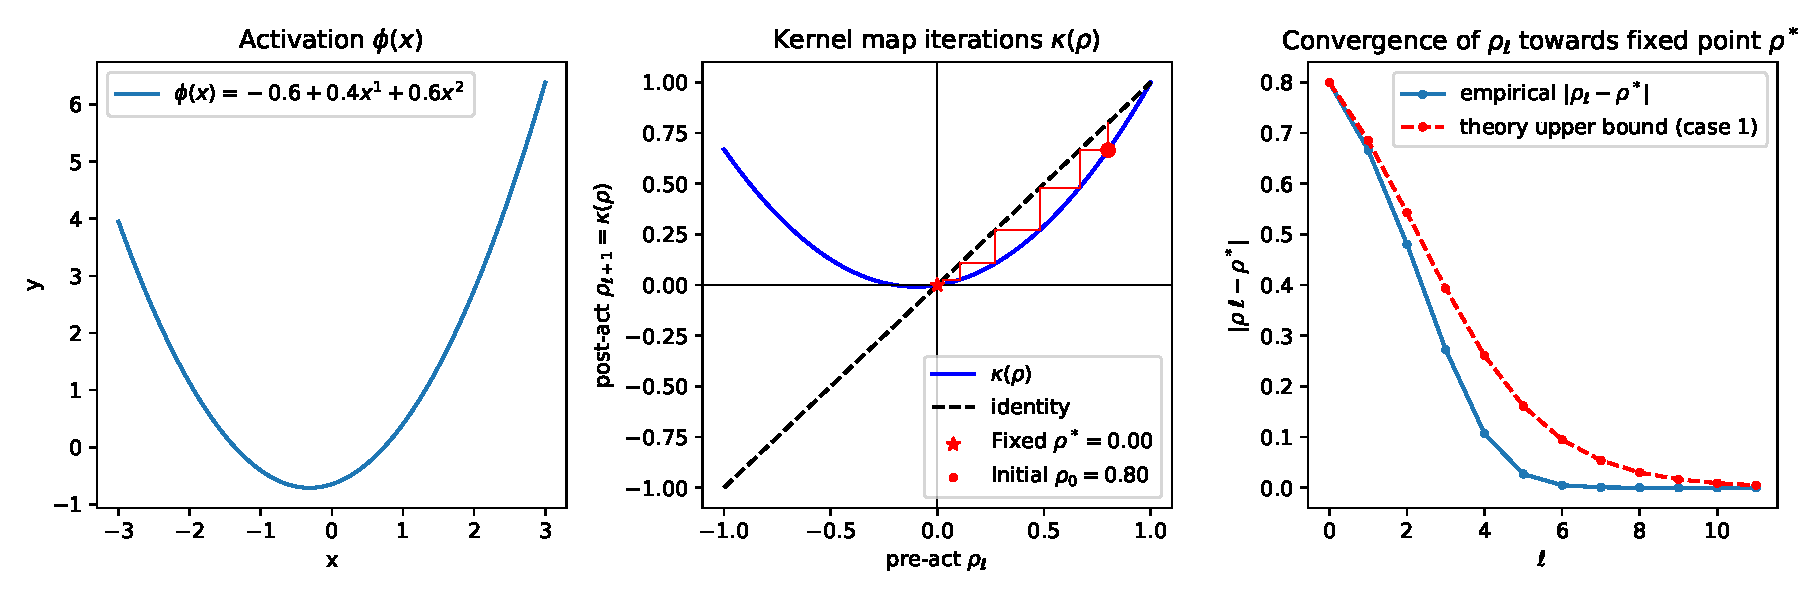
\includegraphics[width=\textwidth]{./kernel_map_convergence_case_0.pdf}
        \caption{\small Case 1}
    \end{subfigure}
    \hfill
    \begin{subfigure}[b]{0.7\textwidth}
        \centering
        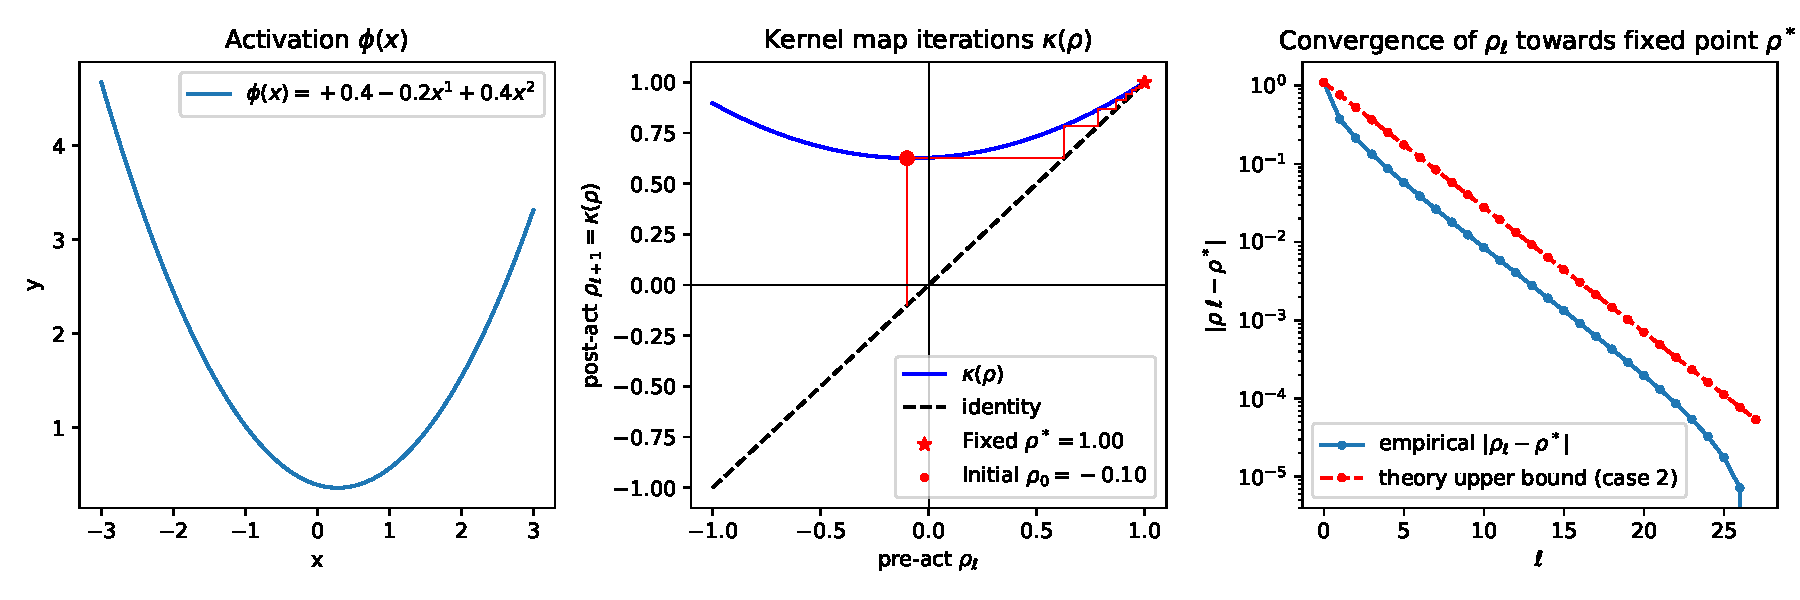
\includegraphics[width=\textwidth]{./kernel_map_convergence_case_1.pdf}
        \caption{\small Case 2}
    \end{subfigure}
    \\
    \begin{subfigure}[b]{0.7\textwidth}
        \centering
        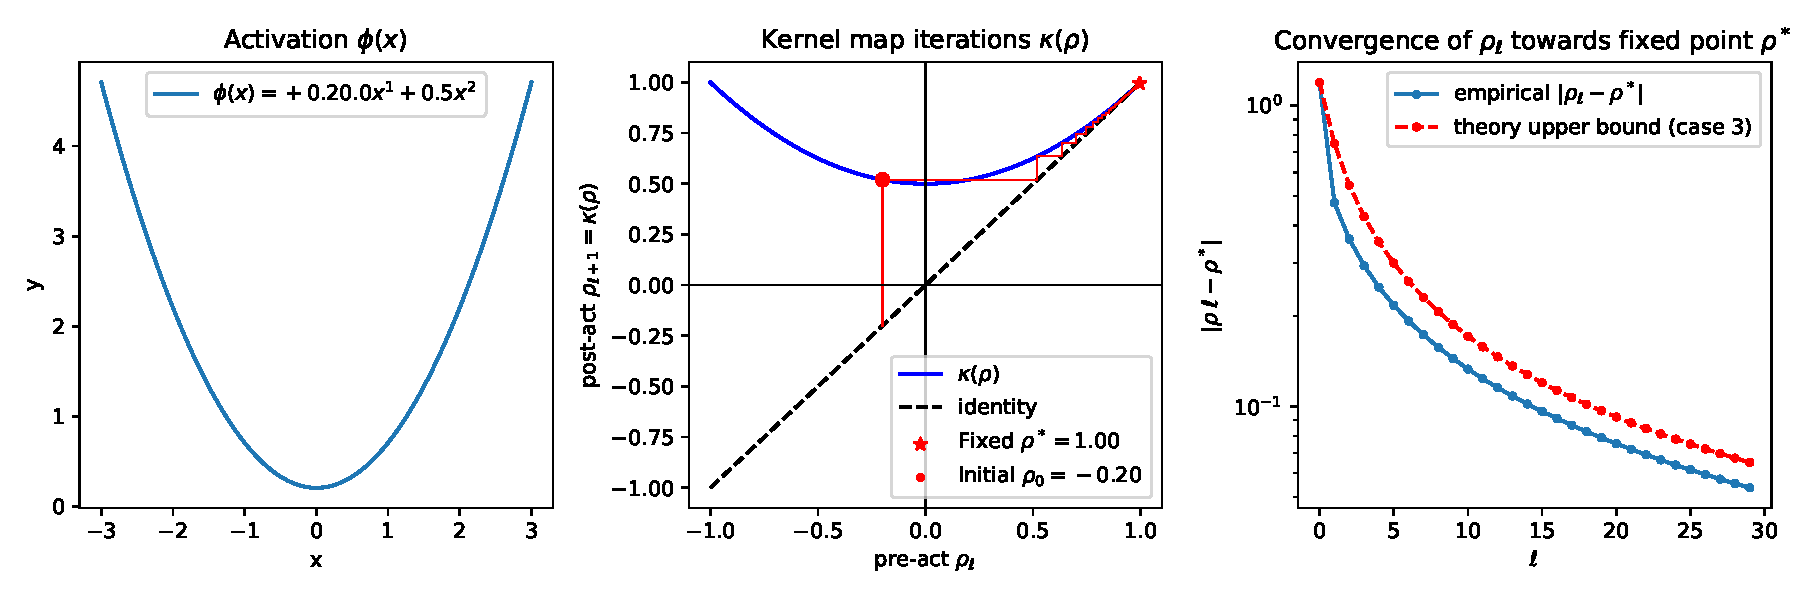
\includegraphics[width=\textwidth]{./kernel_map_convergence_case_2.pdf}
        \caption{\small Case 3}
    \end{subfigure}
    \hfill
    \begin{subfigure}[b]{0.7\textwidth}
        \centering
        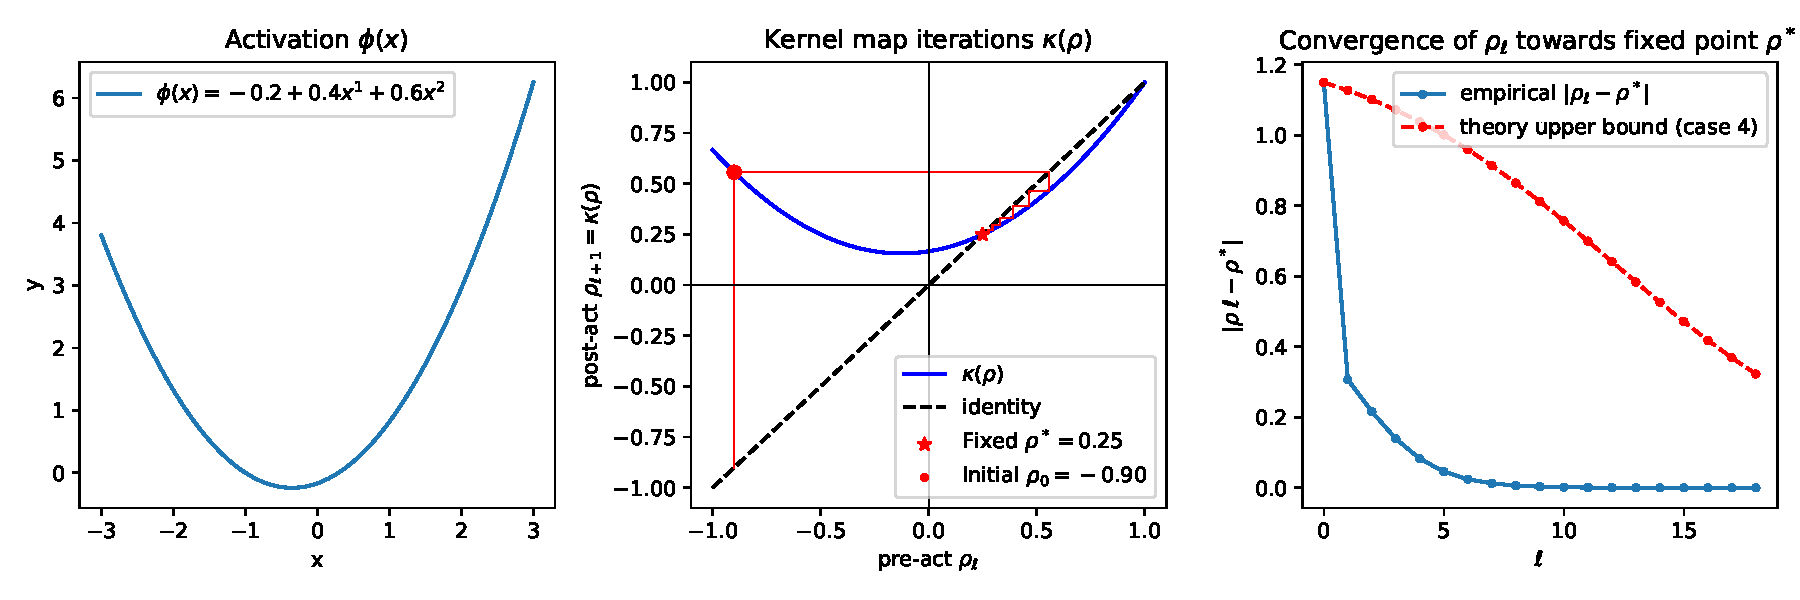
\includegraphics[width=\textwidth]{./kernel_map_convergence_case_3.pdf}
        \caption{\small Case 4}
    \end{subfigure}
    \caption{\small Validation of Theorem~\ref{iso:thm:global_attract}, each corresponding to one of the four cases of the theorem. Left column shows the activation $\phi.$ The middle and right columns show the kernel map show fixed point iteration starting from $\rho_0,$ and applying $\rho_{\ell+1}=\kappa(\rho_\ell)$ for many steps. The middle column shows the kernel map, while the right column shows the distance to the fixed point $\rho^*$.}
    \label{iso:fig:validation_plots}
\end{figure}

\begin{figure}[ht!]
    \centering
    \begin{subfigure}[b]{0.7\textwidth}
        \centering
        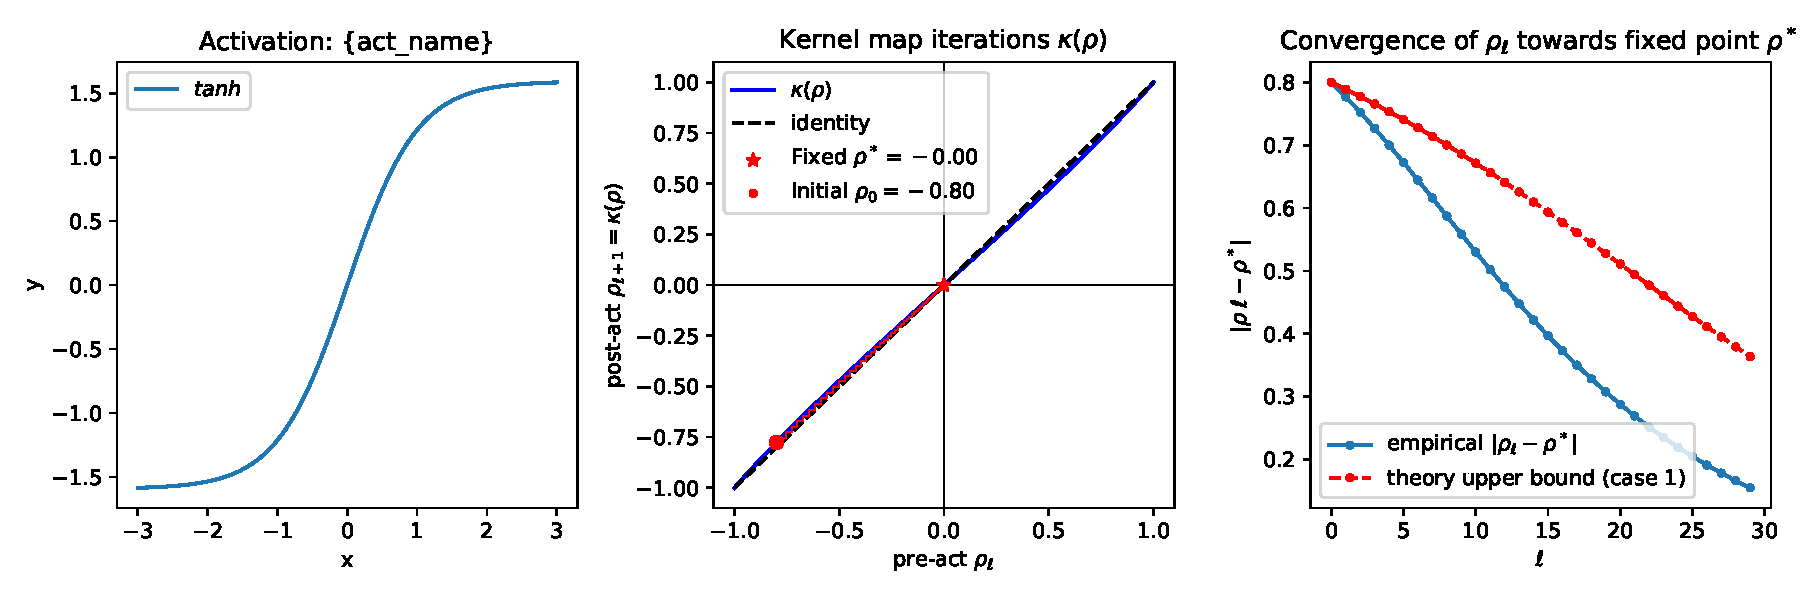
\includegraphics[width=\textwidth]{./kernel_map_convergence_case_0_tanh.pdf}
        \caption{\small Case 1. Tanh activation.}
    \end{subfigure}
    \hfill
    \begin{subfigure}[b]{0.7\textwidth}
        \centering
        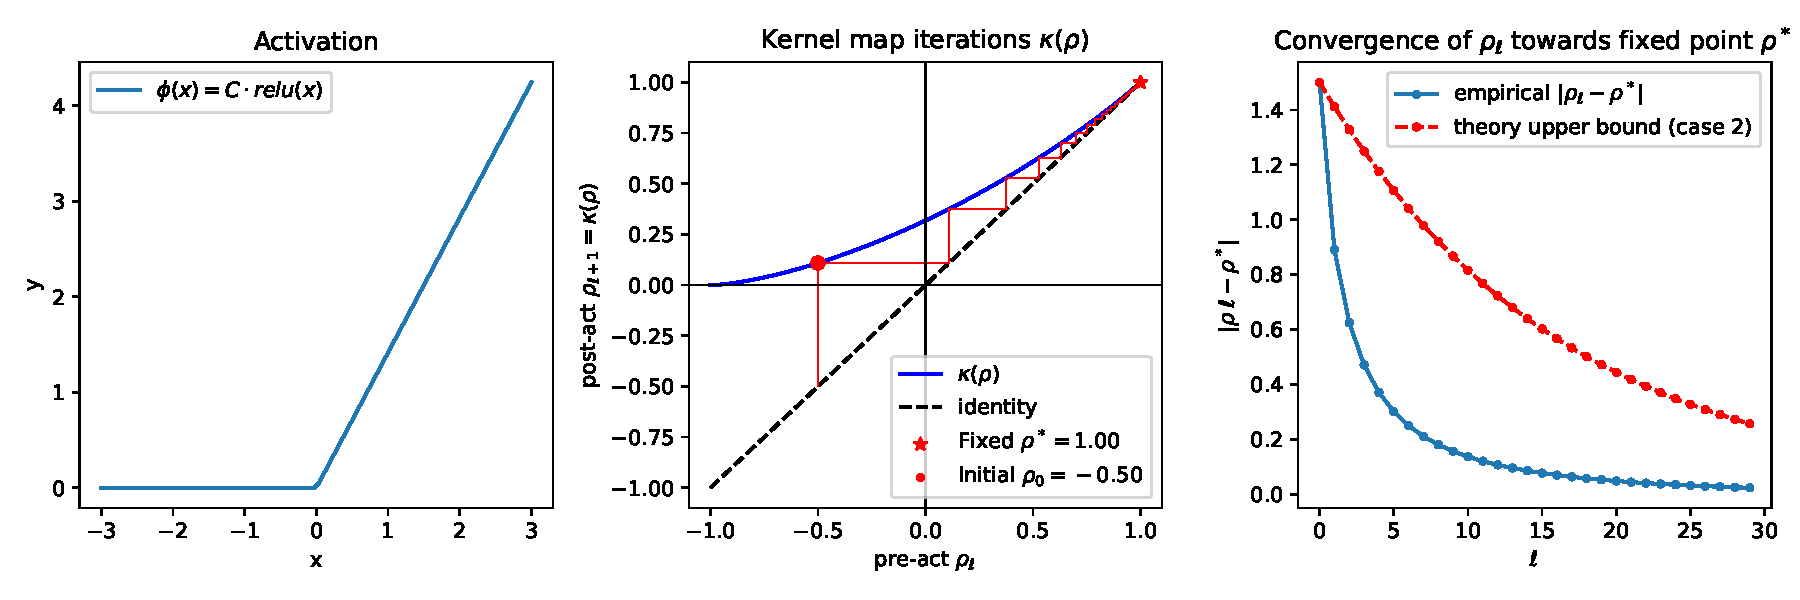
\includegraphics[width=\textwidth]{./kernel_map_convergence_case_1_relu.pdf}
        \caption{\small Case 2: ReLU activation.}
    \end{subfigure}
    \\
    \begin{subfigure}[b]{0.7\textwidth}
        \centering
        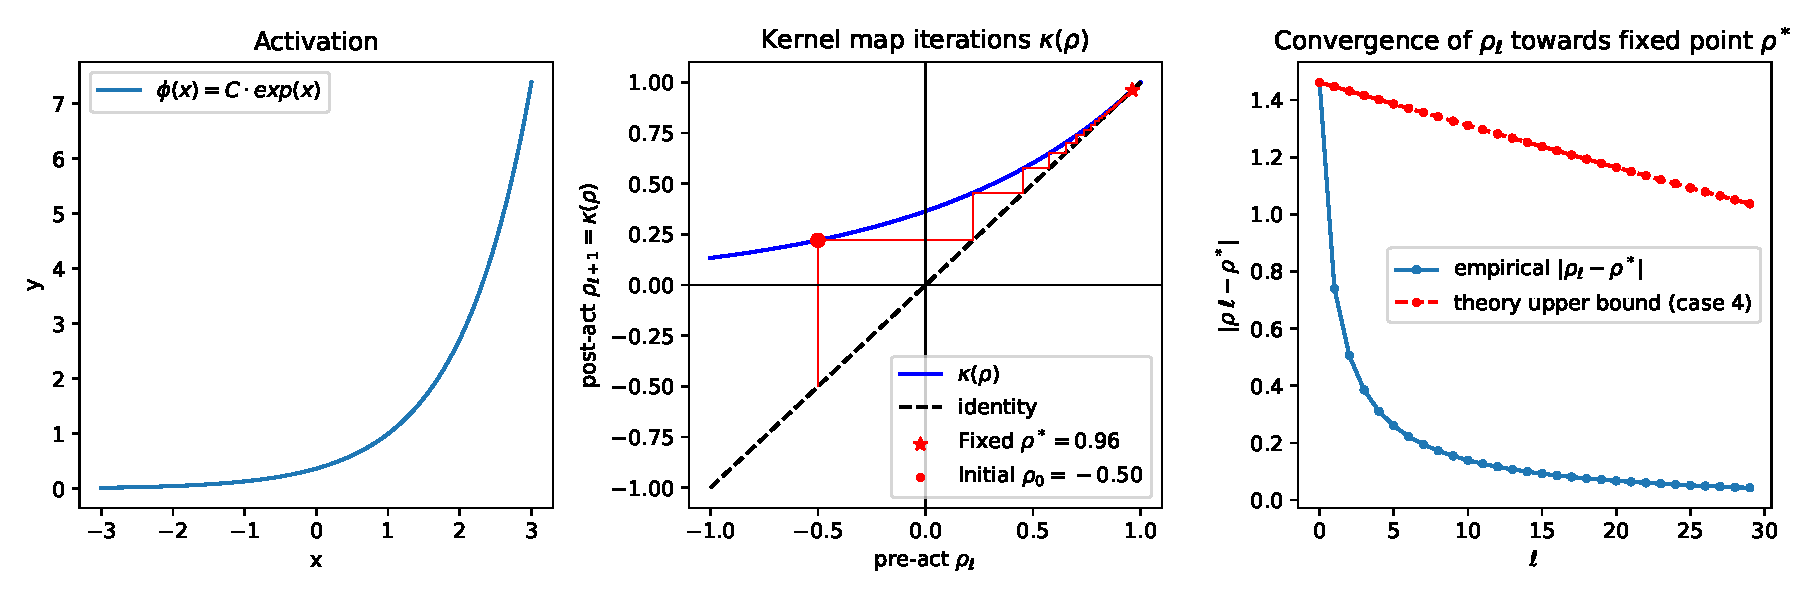
\includegraphics[width=\textwidth]{./kernel_map_convergence_case_2_exp.pdf}
        \caption{\small Case 3: Exponential activation.} 
    \end{subfigure}
    \hfill
    \begin{subfigure}[b]{0.7\textwidth}
        \centering
        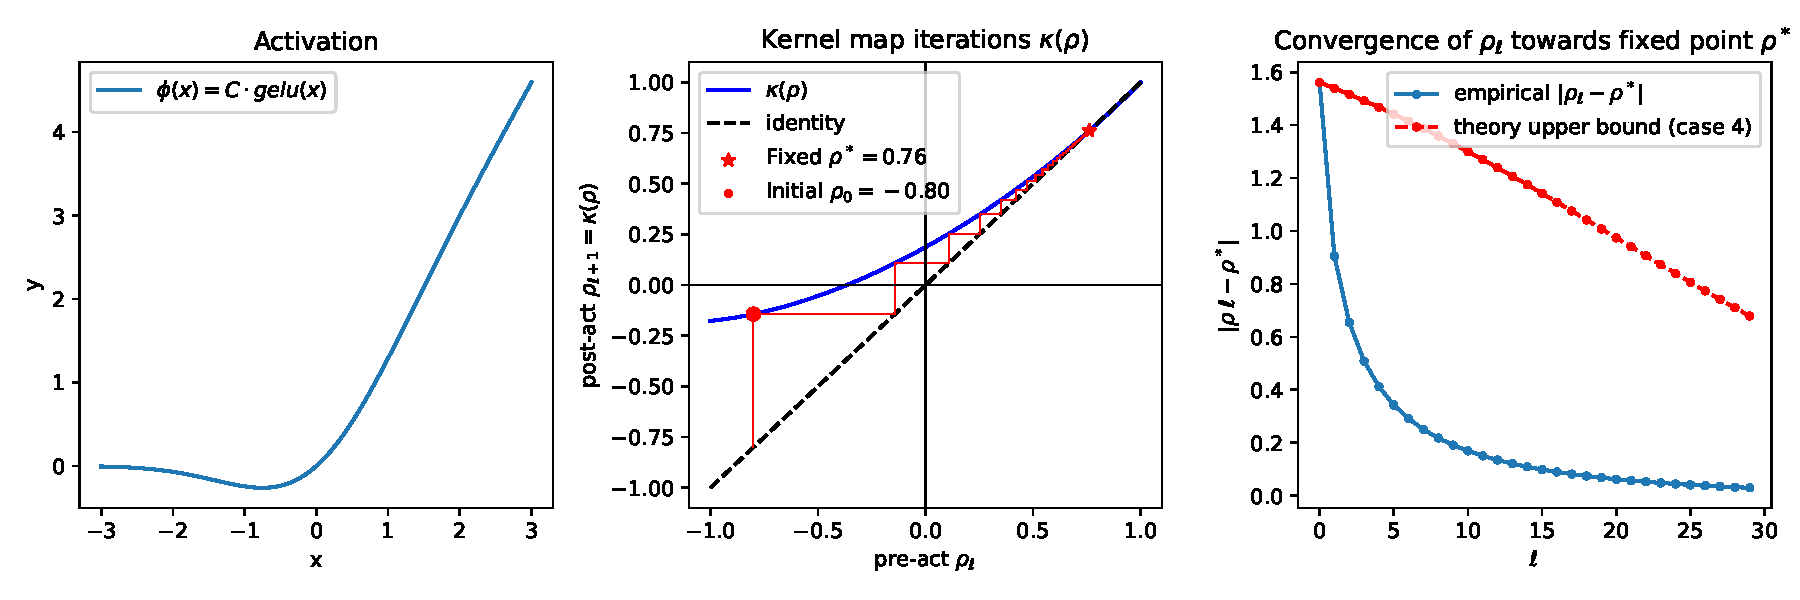
\includegraphics[width=\textwidth]{./kernel_map_convergence_case_3_gelu.pdf}
        \caption{\small Case 4: GELU activation.}
    \end{subfigure}
    \caption{\small Same as Figure~\ref{iso:fig:validation_plots} for some commonly used activations. Note that because the raw activations do not necessariy obey $\E \phi^2(X)=1,$ we have to scale by some contant $C$ to make the activations obey the conditions of the theorem.}
    \label{iso:fig:validation_plots_real_activations}
\end{figure}




% \section{Stability in the non-mean field regime}
% So far, we only considered the mean field regime, where the state of every layer can be exactly determined by conditional expectation of the previous layer. However, when width $d$ is finite, because the sample and population means have some errors, it is not clear how the fixed points of the kernel map will behave. In this section, we will consider stability as the property that if the pre-activations have some deviation from the zero mean, unit variance Gaussian, the post-activations will still converge to the fixed point of the kernel map. In other words, we would like to find out the following dynamics, have locally or globally atracting fixed points:
% \begin{align}
% \mu_{\ell+1} = \E\; \phi(X),\ \sigma_{\ell+1}^2 = \text{Var}(\phi(X)), && X\sim N(\mu_\ell,\sigma_\ell^2),
% \end{align}
% where $\mu_0$ and $\sigma_0^2$ are the mean and variance of the input. Note that if we have centered and properly scaled activation $\E\phi(X)=0, \E\phi(X)^2 = 1,$ then $\mu=0,\sigma^2=1$ are the fixed points of the kernel map. However, in the finite width regime, we would like to know if the fixed points are locally or globally attractive.

% \begin{align}
% &\He_n(x+y) = \sum_{k=0}^n \binom{n}{k}x^{n-k} \He_k(y) \\
% &\He_n(\gamma x) = \sum_{i=0}^{\lfloor \frac{n}{2} \rfloor} \gamma^{n-2i} (\gamma^2 - 1)^i \binom{n}{2i} \frac{(2i)!}{i!} 2^{-i} \He_{n-2i}(x).
% \end{align}

% Thus if $\phi(x)=\sum_{k=0}^\infty c_k\He_k(x)$, for additive purturbation, we have 
% \begin{align*}
% \E_{X} \phi(X+\mu) &=  \E_X \sum_{n=0}^\infty c_n\He_n(X+\mu), && X\sim N(0,1)  \\
% &= \sum_{n=0}^\infty c_n \left(\E_X \sum_{k=0}^n \binom{n}{k}\mu^{n-k} \He_k(X)\right)\\
% &= \sum_{n=0}^\infty c_n \mu^n\\
% \end{align*}
% And for multiplicative purturbation, we have
% \begin{align*}
%     \E_{X} \phi(\gamma X)^2 &= \E_{X}\left(\sum_{n=0}^\infty c_n \He_n (\gamma X )\right)^2\\
%     &=  \E_X \left( \sum_{n=0}^\infty c_n \sum_{i=0}^{\lfloor \frac{n}{2} \rfloor} \gamma^{n-2i} (\gamma^2 - 1)^i \binom{n}{2i} \frac{(2i)!}{i!} 2^{-i} \He_{n-2i}(X)\right)^2\\
%     &= \E \left(\sum_n \He_n(X) \sum_{i=0}^\infty c_{n+2i}\gamma^{n}(\gamma^2-1)^i\binom{n+2i}{2i}\frac{2i!}{i! 2^i}\right)^2\\
%     &= \sum_{n=0}^\infty \left(\sum_{i=0}^\infty c_{n+2i}\gamma^{n}(\gamma^2-1)^i\binom{n+2i}{2i}\frac{2i!}{i! 2^i}\right)^2\E \He_n(X)^2\\
%     &= \sum_{n=0}^\infty n! \gamma^{2n}\left(\sum_{i=0}^\infty (\gamma^2-1)^i \binom{n+2i}{2i}\frac{2i!}{i! 2^i} c_{n+2i}\right)^2\\
%     &= \sum_{n=0}^\infty \sum_{k=0}^n \binom{n}{k}(\gamma^2-1)^k\sum_{i,j=0}^\infty (\gamma^2-1)^{i+j} \binom{n+2i}{2i}\frac{2i!}{i! 2^i}\binom{n+2j}{2j}\frac{2j!}{j! 2^j} c_{n+2j} c_{n+2i}\\
%     &= \sum_{n=0}^\infty \sum_{k=0}^n \binom{n}{k}\sum_{i,j=0}^\infty (\gamma^2-1)^{i+j+k} \binom{n+2i}{2i}\frac{2i!}{i! 2^i}\binom{n+2j}{2j}\frac{2j!}{j! 2^j} c_{n+2j} c_{n+2i}
% \end{align*}

% \section{Gradients and neural tangent kernel}
% So far, we only considered the forward passes. In this section, we consider the backward gradients, which will demosntate the importance of the convergence results that was established in the previous sections. 
% Before that, let us study a few elegant properties of Hermite polynomials that will be useful later.

% \begin{lemma}
% Let $\phi$ be an activation with Hermite expansion $\phi(z) = \sum_{k=0}^\infty c_k \he(z),$ and with kernel map $\kappa.$ Then, its derivative has Hermite expansion 
% \begin{align}
%     \phi'(z) = \sum_{k=1}^\infty \sqrt{k} c_k \he_{k-1}(z).
% \end{align}
%  Furthermore, if $X,Y$ are standard Gaussians with covariance $\rho,$ the kernel map of the derivative is given by 
% \begin{align}
% \E \phi'(X)\phi'(Y) = \kappa'(\rho)= \sum_{k=1}^\infty k c_k^2 \rho^{k-1}.
% \end{align}
% \end{lemma}

% This lemma shows a remarkable property of Hermite polynomilas, in that, the kernel map of derivative, is derivative of the kernel map of the original function. The main proof step is the fact that Hermite polynomials constitute an Appell sequence, i.e., $\He_k'(z) = \sqrt{k} \He_{k-1}(z).$ 

% \begin{proof}
% The derivative of probablist's Hermite polynomials is directly linked tho the lower degree Hermite polynomials, allowing us to write
% \begin{align*}
% \frac{d}{dz} \He_k'(z) = k \He_{k-1}(z) \\
% \implies \he_k'(z) = \sqrt{k} \he_{k-1}(z)\\
% \implies \phi'(z) = \sum_{k=1}^\infty \sqrt{k}c_k\he_{k-1}(z)
% \end{align*}
% Thus, we can conclude the proof by invoking Lemma~\ref{iso:lem:mehler_kernel}
% \begin{align*}
% \E \phi'(X)\phi'(Y) &= \E \left[\sum_{k=1}^\infty \sqrt{k} c_k \he_{k-1}(X) \sum_{k=1}^\infty \sqrt{k} c_k \he_{k-1}(Y) \right]\\
% &= \sum_{k=1,n=1}^\infty \sqrt{k} c_k \sqrt{n} c_n \E [\he_{k-1}(X)\he_{n-1}(Y)]  \\
% &=\sum_{k=1}^\infty k c_k^2 \E [\he_{k-1}(X)\he_{k-1}(Y)]^{k-1} && \text{Lemma~\ref{iso:lem:mehler_kernel}} \\
% &= \sum_{k=1}^\infty k c_k^2 \rho^{k-1} = \kappa'(\rho)
% \end{align*}

% \end{proof}

% Let us now consider the gradients of the MLPs

% \subsection{Gradients of MLPs}
% Given input dimension $d_0,$ output dimension $d_L,$ and hidden dimensions $d_1,\dots,d_{L-1},$ input $x\ni\R^{d_0}$ and output $y\in\R^{d_L},$ the MLP is defined as
% \begin{align*}
% &h^{0} := x, && x\in\R^{d_0}\\
% & z^\ell:=W_{\ell} h^{\ell-1}, && W_\ell\in\R^{d_{\ell}\times d_{\ell-1}},\text{drawn iid from }\sim N(0,1/d) \\
% &h^\ell := \phi(z^\ell), && \ell=1,\dots,L \\
% & \hat{y} := z^{L}=W_L h^{L-1}, && \hat{y},y\in\R^{d_L}
% \end{align*}
% Assuming sum squared, we can deinfe  
% \begin{align*}
% \mathcal{L}(x,y) &= \frac{1}{2} \|\hat{y} - y\|^2,
% \end{align*}
% the gradients of the last layer are given by
% \begin{align*}
% &\delta^{L}:=\frac{\partial \mathcal{L}}{\partial \hat{y}} = \hat{y} - y \\
% &\delta^\ell:=\frac{\partial \mathcal{L}}{\partial z^\ell}= \phi'(z^\ell)\odot (W_{\ell+1}^\top\delta^{\ell+1}), && \ell=1,\dots,L-1 \\
% &g^\ell:=\frac{\partial \mathcal{L}}{\partial W_\ell} = \delta^\ell\otimes h^{\ell-1}, && \ell=1,\dots,L,\\
% \end{align*}
% where $\otimes$ denotes the outer product, and the dependece of $\mathcal{L}$ and $\hat{y}$ on $x$ is omitted for brevity.



% The main goal of this section is to analyze the norm of the gradients in the mean field regime, and then to exend this to the Neural Tangent Kernel (NTK). In other words, we are interested in properties of $\|g^{l}\|_{rms},$ when $d_1,\dots,d_{L-1}\to \infty,$ and wether it vanishes or explodes with the depth of the network. For the NTK, we are interested in the properties of the sequence $\langle g^{l},g^{l}\rangle,$ when $d_1,\dots,d_{L-1}\to \infty.$

% In the remainder of this section, we will use $\rho_{X,Y}$ to refer to average inner product $\rho_{X,Y} = \frac1n \sum_{i=1}^n X_i^\top Y_i.$ Furthermore, we will use $\|X\|_{rms}$ to refer to the RMS norm $\frac1n \sum_{i=1}^n x_i^2.$

% % In this section, we are interested in the gradient norms 
% % \begin{align*}
% % &\text{delta and gradient norms} &&\|\delta^\ell\|_{rms}, \qquad \|g^\ell\|_{rms}, \\
% % &\text{delta similiarty} && \rho_{\delta_1^\ell,\delta_2^\ell}\\
% % &\text{gradient similarity} && \rho_{g_1^\ell,g_2^\ell},
% % \end{align*}
% % where in all cases, $\ell=0$ corresponds to input, and $\ell=L$ corresponds to the output layer, and the indices $1,2$ correspond to two different inputs. Also, recall from previous sections that given two inputs, the kernel sequence for two inputs is given by
% % \begin{align*}
% %     \rho^\ell_h:=\frac{\langle h_1^\ell,h^\ell_2\rangle}{\|h_1^\ell\|\|h_2^\ell\|},
% % \end{align*}
% % where $\ell=0$ corresponds two different inputs. 


% \begin{proposition}
%     Let $\phi$ be an activation that obeys $\E_{X\sim N(0,1)}\phi(X)^2=1.$ In the mean field regime, the norm of the gradients obeys
%     \begin{align}
%         \|\delta^\ell\|_{rms} = \|\delta^{\ell+1}\|_{rms} \kappa'(1)
%     \end{align}
%     Furthermore, for two inputs with initial similarity $\rho_0 = \langle x_1,x_2 \rangle $ the forward and backward passes follow recursion
%     \begin{align}
%         &\rho_\ell:=\rho_{h^\ell_1,h^\ell_2} = \kappa(\rho_{\ell-1})\\
%         &\langle \delta_1^\ell,\delta_2^\ell \rangle = \kappa'(\rho^\ell) \langle \delta_1^{\ell+1},\delta_2^{\ell+1} \rangle \\
%         &\langle g^\ell_1,g_2^\ell \rangle =\rho^{\ell-1}   \langle \delta_1^{\ell},\delta_2^{\ell} \rangle.
%     \end{align}
% \end{proposition}

% Let us consider the backward errors $\delta^{l}$ and their norms. Each index of $\delta^{l}$ is a Gaussian weights at layer $l+1$, by $\delta^{l+1}$ and $\phi'(z^{l}).$ Conditioned on the norm of $\delta^{l+1}$, with the independece of weights of at layer $l+1$ and pre-activations at layer $l$, norm of $\delta^{l}$ is the multiplication of norm of $\delta^{l+1}$ and the norm of $\phi'(z^{l}).$ Now, assuming that the activation is centered, pre-activations are standard Gaussian, and thus $\E \phi'(z^{l})^2 $ can be expanded based on the Hermite expansion and properties of Hermite polynomials 
% \begin{align*}
% &\phi'(z) = \sum_{k=1}^\infty c_k \he_{k-1}(z)\\
% &\E \phi'(z^{l})^2 = \sum_{k=1}^\infty \frac{c_k^2}{k}=:\beta\\
% &\|\delta^{l}\|_{rms} = \|\delta^{l+1}\|_{rms} \E \phi'(z^{l})^2 = \|\delta^{l+1}\|_{rms}\beta\\
% &\|\delta^{l}\|_{rms} = \|\delta^{L}\|_{rms} \beta^{L-l} = \|y-\hat{y}\|_{rms} \beta^{L-l}
% \end{align*}

% \begin{remark}
% Note that assuming that the activation unit second momnt $\E\phi(X)^2=1,$ we have $\sum_{k=1}^\infty c_k^2 = 1,$ which implies that $\beta \le 1.$ Furthermore, if the activation is non-linear, i.e., there is $c_k\neq 0$ for some $k\ge 2$, then the inequality is strict, i.e., $\beta < 1.$ 
% Recall that for the forward pass of an activation that centered and unit variance, we have shown the the kernel sequence converges towards zero with rate $\alpha = 1/(\sum_{k=1}c_k^2),$  where the rate becomes strict whenever we have any non-linearity. 
% This implies that the stronger the non-linearity, the faster the convergence of kernel sequence towards zero, and the faster the gradients norms converge towards zero. This shows that striking a balance between linearity and non-linearity is probably needed for a desirable initialization.
% \end{remark}


% Now, consider a generic layer $\delta' = \mathbf{W}^\top \delta \odot \phi'(\mathbf{z})$. Suppose $z_1,z_2 $ correspond to pre-activations for two different inputs, and $\delta_1,\delta_2$ are the corresponding gradients for previous and $\delta_1',\delta_2'$ are the gradients for the next layer. 

% If we look at one corresponding unit of $W_\top \delta_1$ and $W_\top \delta_2,$ they are jointly Gaussian with covariance $\E \delta_1\delta_2 .$ Thus, in the mean field, we can write
% \begin{align*}
%     \E \delta'_1\delta'_2 =  (\E \delta_1 \delta_2)(\E \phi'(z_1)\phi'(z_2)) 
%     = \E \delta_1\delta_2 f(\rho),
% \end{align*}
% where we used the fact that error-propagation vectors $\delta_1\delta_2$ are independent of pre-activations $z_1 z_2,$ because one relies on layers before and the other on layers after this step. 

% Now, in a multi-layer setting, let $r_l = \frac1d\langle \delta_1^{l},\delta_2^{l}\rangle$ denote the normalized inner product of the gradients at layer $l$, and let $\rho_\ell = \frac1d \langle z^{l}_1,z_2^{l}\rangle$ denote the normalized inner product of the pre-activations at layer $\ell$. Then, in the mean field regime, we have
% \begin{align*}
%     r_l = f(\rho_l) r_{l+1}
% \end{align*}
% Thus, for the weight gradients of layer $\ell$, we have


% \section{Limitations and open questions}

% The main theorem of this chapter, which was the global contraction towards zero, was only for the centered activations. However, there are possibly other fixed points. This question was not addressed in this chapter. 

% There is one conjecture that seems to be true but remained out of the scope of the results of this chapter:

% \begin{conjecture}
%     For any activation function $\phi$ that satisfies $\E_{X\sim N(0,1)}\phi(X) = 1,$ and is nonlinear, the following is true for the fixed-points of the kernel map :
%     \begin{itemize}
%         \item There are no fixed points in the range $(-1,0).$
%         \item There is exactly one fixed point in the range $\rho^*\in [0,1],$ that obeys $\kappa'(\rho^*) < 1,$ and it is globally attracting.
%     \end{itemize}
% \end{conjecture}



% \section{Implications for backward pass of MLPs}

% So far, we have only discussed the theory for the forward pass of neural networks. In this section, we will briefly discuss their implications for the backward pass. To the best of our knowledge, this connection has not been explored in the literature.

% \begin{proposition}
% Given an MLP with activation $\phi$ that has unit gain, in the mean field regime, the second moment of the eigenvalues of the Jacobian $J^\top J$ will be approximately $(\kappa'(1))^\ell$, which can be viewed as the backward gain of the activation function, $\kappa$ is the kernel map, and $\ell$ is the number of layers.
% \end{proposition}

% \begin{proof}
% Consider our principal result on the kernel map, which relates the covariance of pre-activations to the covariance of post-activations:

% \begin{align*}
% \kappa(\rho) = \E_{X,Y}[\phi(X)\phi(Y)] \quad \text{for } X,Y\sim \mathcal{N}(0,1) \text{ with covariance } \rho = \E[XY].
% \end{align*}

% Let us consider the scenario where the two signals are arbitrarily close, i.e., $\rho = 1- \epsilon$. In such a scenario, the kernel map  will be:

% \begin{align*}
% \lim_{\epsilon\to 0}\frac{\kappa(1)-\kappa(1-\epsilon)}{\epsilon} = \kappa'(1).
% \end{align*}

% This reveals that for a small $\epsilon$-perturbation in the covariance of pre-activations, the covariance of post-activations will be perturbed by $\kappa'(1)$-factor larger. We define this coefficient $\kappa'(1)$ as the backward gain of the activation function. In a multi-layer setting with $\ell$ layers, the gain will be $(\kappa'(1))^\ell$.

% Now, let's interpret this result using the definition of derivative. Consider an input $x$ and a small perturbation $\delta$. The output will be:
% \begin{align*}
% &h^\ell(x+\delta) = h^\ell(x) + J\delta, && J=\partial h^\ell(x)/\partial x,
% \end{align*}
% where $J$ is the input-layer-$\ell$ Jacobian. Thus, we can write:
% \begin{align*}
% \| h(x+\delta)-h(x)\| = \|J \delta\|.
% \end{align*}
% The backward gain in this sense will be $\|J \delta\|/\|\delta\|$.

% If we consider the case where the $\delta$ orientation is randomly chosen from a unit sphere, the distribution of $\|J \delta\|^2$ will be tightly related to the eigenvalue distribution of $J^\top J$. Specifically, its second moment will be:

% \begin{align*}
% \E_{\delta\sim \mathbf{S}^{d-1}} [\|J \delta\|^2] 
% = \frac1d \E_{\delta\sim \mathbf{S}^{d-1}} \sum_{i=1}^d \delta_{i}^2\lambda_i(J^\top J)\\
% =  \frac{1}{d} \sum_{i=1}^d \lambda_i(J^\top J).
% \end{align*}

% From our earlier analysis, we expect this quantity to be around $(\kappa'(1))^\ell$. Therefore, we can conclude that the second moment of the eigenvalues of $J^\top J$ will be approximately $(\kappa'(1))^\ell$, connecting our analysis of the backward pass to the Hermite expansion of the activation function.
% \end{proof}



